\documentclass[a4paper,11pt]{article}
\usepackage{array}
\usepackage{tabularx}
\usepackage{booktabs}
\usepackage{graphicx}
\usepackage{framed}
\usepackage{comment}
\usepackage{spverbatim}
\newcommand{\ra}[1]{\renewcommand{\arraystretch}{#1}}
\newcommand{\specialcell}[1]{\begin{tabular}{@{}c@{}#1\end{tabular}}}
\newcommand{\CS}{C\nolinebreak\hspace{-.05em}\raisebox{.6ex}{\tiny\bf \#}}
% define the title
\author{StroustrupSekten}
\title{Slice of Pie}
\begin{document}
\maketitle
\section{Preface}
\newpage
\tableofcontents
\newpage
\section{Abstract}
\newpage
\section{Introduction}
In this report, we will cover central topics of the Analysis, Design and Software Architecture course (BDSA) as we have applied them to our project during the Fall of 2012.\\
\newline
The report documents our activities ranging from our usage of the Rational Unified Process (RUP) artifacts \cite[p.~31]{OOAD} to our usage of the Scrum methodology to manage our agile development. Moreover, we will discuss several C\# technologies and how we have applied them to make our proof of concept.\\
\newline
After a brief introduction to Scrum, we have structured this document as a series of sprints (timeboxed periods of incremental development), each documenting our steps towards release date (the project delivery date). The report is structued this way to give a better view of the iterative process and show where in the process we have utilized the different software engineering tools and processes.\\
\newline
Because of the limited time we have to do the project we have decided to limit ourselves to the following three sprints:\\
\begin{itemize}
\item An introductory sprint, in which we focus a lot on major design and architectural decisions as well as programming some high-risk elements on our system
\item A longer, ‘elaboration’ sprint in which we focus on detailed design and analysis of major components as well as connecting important sub-systems 
\item Finally, a release sprint, in which we fine tuned selected components as well as made the adjustments to our documentation to make it a documentation of a product as well as a process.
\end{itemize}
In each sprint, we will describe the artifacts created in the sprint. However,
we would like to note two things relevant to the structure of our report:\\
\begin{enumerate}
\item The order of which the artifacts appear in the sprint is not necessarily equal to the
  order in which they were created (internally in the sprint). Each artifact
  may be created and revised several times during a sprint as it is relevant
  to the understanding of a design or a requirement. 
\item Not all reviews and revisions of the artifacts are described in the
  report. Only significant changes to an artifact or any change we find to have particular value will be highlighted.
\end{enumerate}
\subsection{Scrum}
As mentioned in the previous section, we will use the Scrum method to manage iterative development. Before we cover the actual sprints, we will present an overview of Scrum and the Scrum activities we will do the in sprints.
\newline
Scrum is an iterative framework designed to manage software development projects \cite{scrumguide} \\
The methods originally intends to include a team of up to eight persons, along with a Scrum Master and a Product Owner. However, as we were only five persons we had no choice but to appoint these roles to team members. Moreover, we decided that we wanted a more democratic approach to the features that we included in our project; this implied that the responsibility of creating product backlog items were spread out on the whole group instead of relying solely on the Product Owner \cite[p.~12]{scrumguide}.
\subsubsection{Daily Scrum}
According to the Scrum methodology, each full workday (in all sprints) is initiated with a daily Scrum. In this 15 minute meeting, we each report how progress is made with each task that is on the product backlog. Moreover, each team member can request help from other member in regards to difficult tasks. We use the Task Board of our Scrum tool as our primary form of task management. Each team member is standing up as to signal the immediate focus needed to do an effective meeting. In any case where a team member need some help, the Scrum Master either immediately facilitate the help needed (e.g declaring another members to a particular task) or he undertakes the responsibility to get the help needed later. Below is a picture a of a Scrum meeting with all members standing up around the Task Board, which is projected on a canvas.
\begin{figure}[H]
  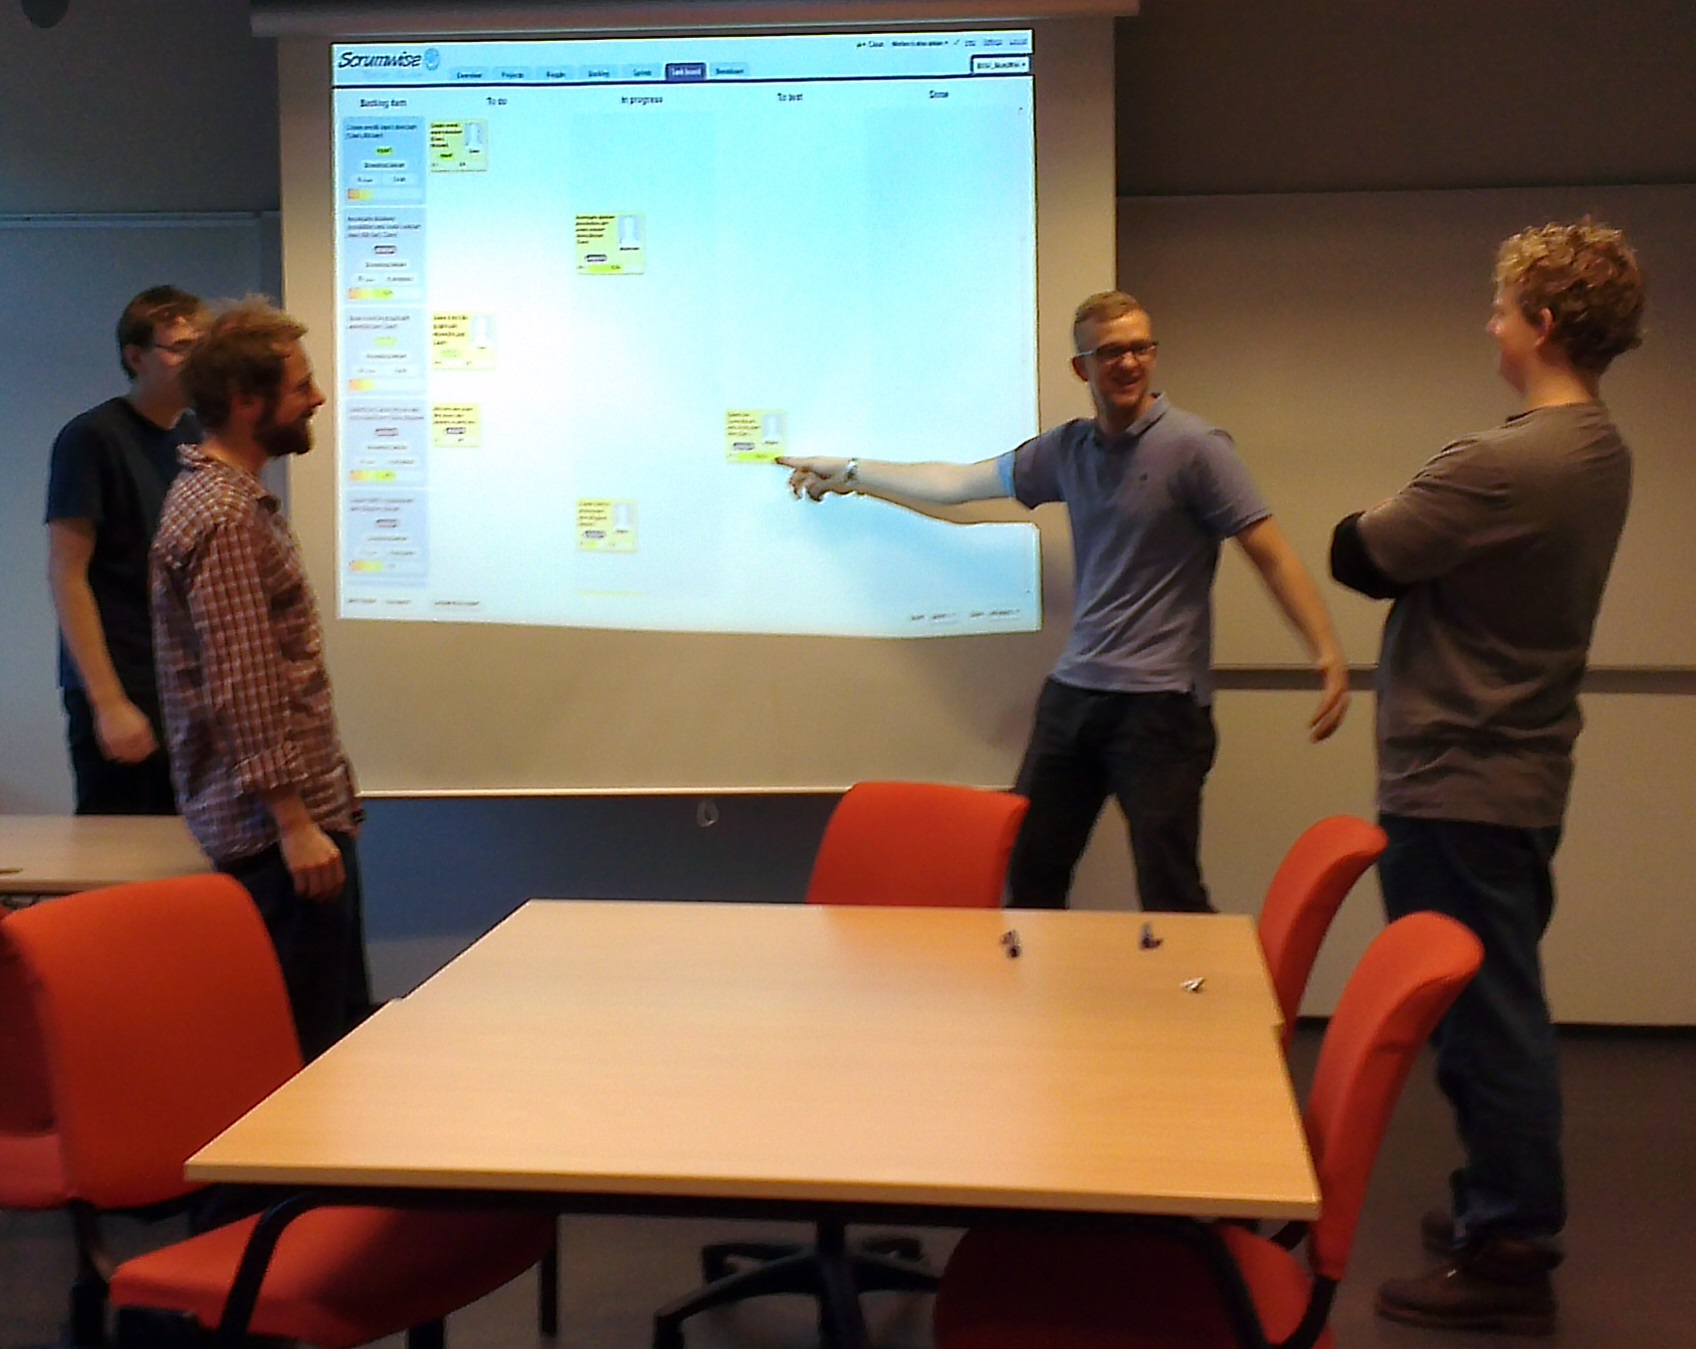
\includegraphics[width=\textwidth,natwidth=1696,natheight=1349]{illustrations/Daily.jpg}
  \caption{Daily Scrum}
  \label{dailyscrum}
\end{figure}
After the Daily Scrum, the Scrum Master reviews the burndown chart for the sprint and compares it to the release date. 
\subsubsection{Sprint planning}
The Sprint planning meeting is the planning of the upcoming sprint. The different stories in the product backlog are prioritized. It is decided which tasks the sprint should consist of and the workload capacity of each team member is determined.
\subsubsection{Sprint review}
The review is the process of reviewing the work that has been done in the sprint, with focus on the the backlog items. The main goal of this activity is to measure the project against the goals determined in the sprint-planning.
\subsubsection{Sprint retrospective}
In conclusion of the scrum activities, we do a Scrum Retrospective. The retrospective mainly focuses on reviewing the process of doing Scrum, as opposed to the concrete backlog items. The main goal of this activity is to increase the productivity of each sprint iteratively by actively inspecting each Scrum related activity.
\section{Scrum}
\subsection{Definition of Done}
\subsubsection{General}
\begin{itemize}
  \item Must be reviewed and accepted by another team member
  \item Story must be completed from beginning to end
\end{itemize}

\subsubsection{Documentation}
\begin{itemize}
  \item Must be in digital form
\end{itemize}

\subsubsection{Program}
\begin{itemize}
  \item Proper documentation has been written. This includes full documentation for public methods
  \item Tests have been written and they they do not fail
  \item New code must not break previously written tests
\end{itemize}
\newpage
\section{Sprint 1: First iteration}
In this section, we will present and discuss the development that took place in the first iteration of our project. This includes a relevant presentation of the Scrum methodology as we have applied it in the sprint. We will mostly present artifacts created that are relevant to the inception and elaboration phases of the unified process.
\subsection{Scrum}
Scrum is an iterative framework designed to manage software development projects \cite{scrumguide} \\
The methods originally intends to include a team of up to eight persons, along with a Scrum Master and a Product Owner. However, as we were only five persons we had no choice but to appoint these roles to team members. Moreover, we decided that we wanted a more democratic approach to the features that we included in our project; this implied that the responsibility of creating product backlog items were spread out on the whole group instead of relying solely on the Product Owner \cite[p.~12]{scrumguide}.
\subsubsection{Initial Scrum}
Before initializing our first sprint, we decided to conduct two sprint planning meetings in somewhat extended versions. Since this were our first project in which we’ve used Scrum, we decided that we would ignore the time bounds that are specified in the Scrum guide \cite[p.~9]{scrumguide}. This allowed us to discuss and familiarize ourselves with the Scrum concepts.\\
The initial meetings were divided into several parts: First, we agreed on using the Scrumwise \cite{scrumwise} tool for organizing our Scrum activities. Then, we all democratically built the product backlog. \\
An important part of the formation of our team before the first sprint were also doing a formal written definition of done. This includes defining a strategy for testing, coding, documentation and acceptance from the rest of the team. The definition of done can be viewed in [Appendix, \ref{defdone} and \ref{deftesting}, page \pageref{defdone} and \pageref{deftesting}].\\
% add ref
Lastly, we had to agree on the number and length of the sprints we were going to do. This also meant creating an overall timeline of the sprints, which can be viewed in [Appendix Figur [sprinttimeline.jpeg]  These initial exercises allowed us to conduct the two, more formally defined meetings of sprint planning: part one of two, respectively. \\
A partial view of the product backlog can be found in Appendix, Figur \ref{backlog1}, page \pageref{backlog1} \\
%ref
\subsubsection{Sprint planning $|$ \& $\|$}
After our initial Scrum agreements, we conducted planning meeting part one for the next sprint. This involved several noteworthy items:
\begin{itemize}
\item Creating a capacity plan to get an overview of our initial work capacity [Appendix, Figur \ref{capacityplan}, page \pageref{capacityplan}]
%  ref
\item Estimating difficulty and priority of the items on the Product Backlog
\item And elaborating on the meanings of the different backlog items to each other (as part of not having a single product owner).
\end{itemize}
Then moving on to the second part of the meeting, where the team were:
\begin{itemize}
\item committing to highest prioritized tasks and estimating their time to complete
\item distributing the work so the workload was fair on each individual
\item initialize the sprint in the Scrumwise tool and review the burndown chart generated
\end{itemize}
An overview of the first Sprint Backlog is available in [Appendix, Figur \ref{sprint1backlog}, page \pageref{sprint1backlog}].\\
% ref
It is worth nothing that even though we decided on all having influence on the product backlog, the management of the backlog were deferred to one person, the “Product Owner”.\\
\subsubsection{More Scrum}
Our Scrum workflow also covers doing following exercises:\\
\begin{itemize}
\item Doing Daily Scrum meetings, updating burndown charts and reviewing our task boards
\item Updating our product backlog during the sprint so tasks are ready for next sprint
\item Doing the Scrum retrospective and review
\end{itemize}
However, we’ve chosen to defer the description and discussion of these exercises to later sprints where we think they’re more relevant.

\subsection{Initial Software Analysis}
This section will cover our initial analysis of the requirements as given in the project description [reference: project description]. We will describe different RUP artifacts created during the process, such as Use Cases, Domain Model, System Sequence Diagrams and Supplementary Requirements.\\
Please note that in the spirit of agile development, the artifacts created in the first sprints are incomplete and draft-like in appearance. The artifacts are then extended and reviewed in later iterations as the need for understanding them increases.\\
\subsubsection{Domain Model and Relational Model}
Before doing any design of the system, we realize the need for a common terminology to describe our understanding of file-sharing and document handling applications. We make a crude initial domain model in order to discuss our understanding of each entity:\\
\begin{figure}[H]
  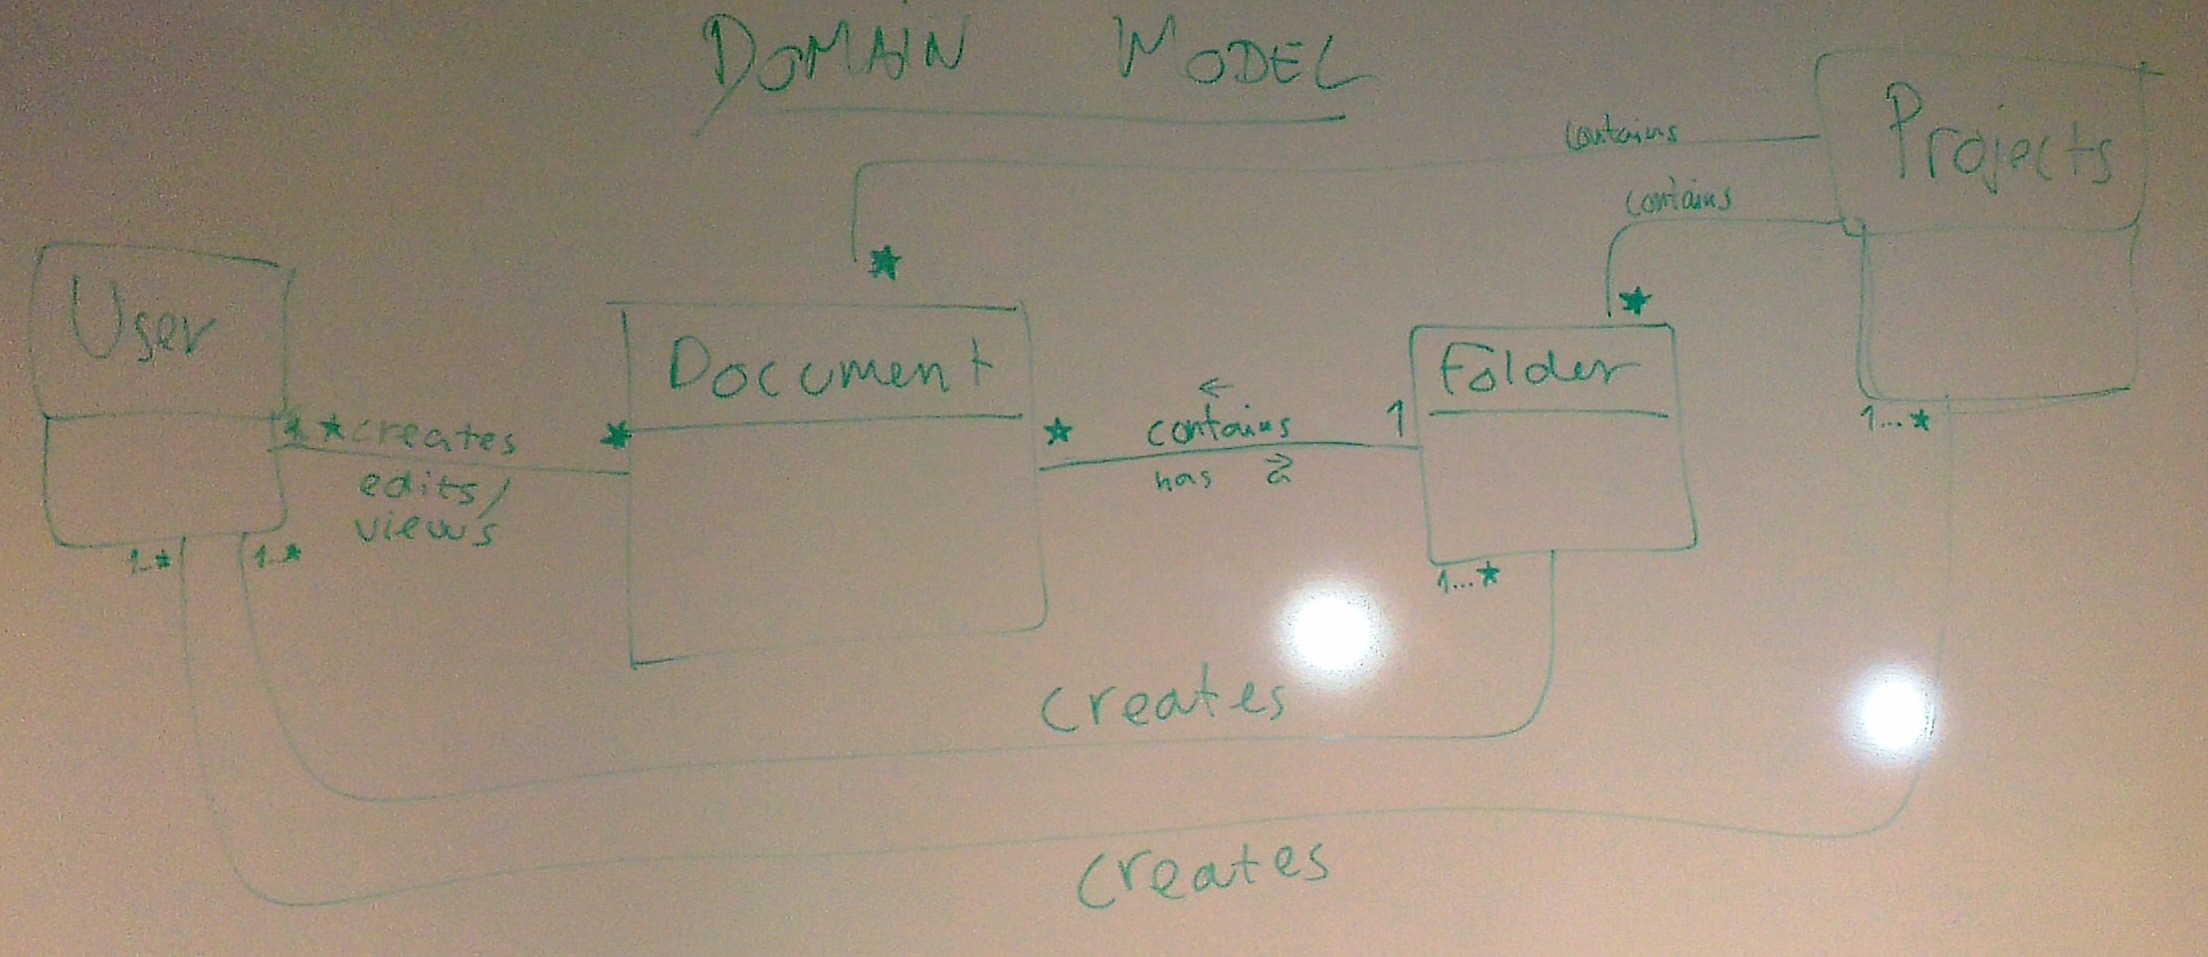
\includegraphics[width=\textwidth,natwidth=2208,natheight=957]{illustrations/DomainModel.jpg}
  \caption{Domain Model}
  \label{domainmodel}
\end{figure}
The picture shows our first draft of the domain model. It shows that our domain model reflects the entities needed to fulfill the requirements given in the project description.\\
Additionally, we quickly identify that online storage using a database will be an important part of our system. As a consequence we also add a relational data model to create a better view of the entities in this aspect:\\
\begin{figure}[H]
  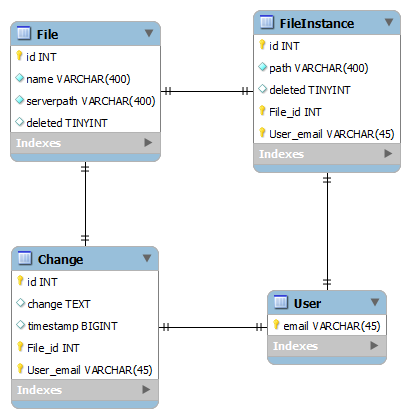
\includegraphics[width=\textwidth,natwidth=410,natheight=418]{illustrations/RelationalData-model.png}
  \caption{Relational Data-Model}
  \label{relationalmodel}
\end{figure}
As it clearly shows, both of these models were quickly drawn and used primarily for their discussion value. The relational model also covers changes made to a document, which we did not include in the initial domain model.\\
Later, we will review both models as they are expanded to support the requirements.\\
\subsubsection{Requirements Analysis with Use Cases}
Before analyzing any requirements, a reasonable exercise could be to create a vision for the product to develop \cite[p.~58]{OOAD}. However, as the high level requirements were already defined in the project description, we decide to skip this artifact.\\
\newline
Understanding the requirements means creating different artifacts that helps develop early ideas of how to solve each requirement. We write down several use cases in a brief form, only covering 1) the goal of the use case and 2) brief explanations of scenarios. A few of the use cases are expanded to include an extended description of alternate case flows as well as pre- and postconditions. Below is an example of a brief use case, ViewVersionHistory:\\
\newline
% [UseCase #4 here in cursive as a quote and delete it from appendix].  
\texttt{USE CASE \#4: VIEW VERSION HISTORY\\
The user wants to view a history for a file in the Slice Of Pie system. He will select a file from the graphical user interface in the system and click on a show version history button. The system will retrieve version history for the file and display it in a new window. \\
ALTERNATE:\\
The user wants to revert document to an earlier state. This use case has yet to be defined and elaborated on.}\\
% Margin?
\newline
The example shows a Use Case detailing the process of viewing a version history of a file.
The use cases created in this sprint are shown in [Appendix, Use Cases page \pageref{usecases}].
% ref
\subsubsection{Non-trivial requirements}
To further elaborate on requirements that may require complex implementation in the system, we create additional artifacts to understand them. The example we will show here is the users ability to synchronize documents between a client and the server holding the documents in online storage. To illustrate the interaction between the user and the system when this process is occurring, a System Sequence Diagram is drawn to display this [Appendix, Illustrations, Figur \ref{activitydiagram}, \pageref{systemsequencediagram}]. The SSD is shown in the Appendix.\\
Moreover, to elaborate on the conditions of the requirement, we create an Operation Contract as shown below:\\
\begin{table*}[ht]\centering
  \ra{1.3}
  \begin{tabularx}{\textwidth}{@{}rXXl@{}}\toprule
    \textbf{Contract CO1:} & SynchronizeWithServer\\
    \textbf{Cross References:} & Use Case \#2: Synchronize\\
    \textbf{Preconditions:} &  The user has an internet connection. The server is up and running.\\
    \textbf{Postconditions:} & The user has received files made in another client application.\\
    & The client has sent files to online storage.\\
    & The user interface displays the newly received files.\\
    \bottomrule
  \end{tabularx}
\end{table*}
The artifacts described above serves to make the requirement explicit and well-defined. The requirement is purely functional, however, and does not specify any measurable quality factors on the Use Case such as: how fast the process should be, how we should handle errors etc. However, trying to elaborate on all requirements is a time-consuming process and as RUP suggests \cite[12.2 p.~196]{OOAD}, we will instead start implementing the high-risk elements of the requirements, then review and adapt the requirements at a later iteration. \\
\subsubsection{Supplementary Specification}
As part of the initial analysis, it is suggested by RUP that a coarse supplementary specification is started in the inception of the iterative development \cite[7.1 p.~102]{OOAD}. Hence, we create an outline of the non-functional requirements in a Supplementary Specification. The non-functional requirement is presented as the FURPS+ checklist. The main reason for this specification is the impact the non-functional requirements may have on the logical architecture of the system.\\
\newline
The Supplementary Specification concludes our artifacts created as part of the initial analysis. These artifacts are mainly supposed to provide a base for our initial code design and choice of logical architecture.\\
\subsection{Initial Design and Architecture}
This section covers our initial program design. We will show the artifacts related to the process of choosing a logical architecture and their influence. Moreover, we'll describe and discuss Class Diagrams as our layers in our architecture were initially thought out. 
% [maybe we need some more introduction here]
\subsubsection{Logical Architectural Design}
% refs following
Our initial logical architectural design signals a transition from understanding and analysing the requirements to actually outlining major subsystems of the program. This is done with the artifacts from earlier described in mind.\\
The requirements explicitly state that the program should contain two modes of program execution: offline and online work. Hence, in order to use several features of the .NET framework we decide to make separate User Interfaces to support this. It follows that we need some separation between UI and the logic applied when synchronizing documents between applications as according to the Model-View separation Principle \cite[p.~209]{OOAD}. Additionally, we want to introduce a layer between persistence of the documents and the synchronization logic specific to the client or the server. Outlining this initial architecture is a very crude UML package diagram as shown in [Appendix, Figur \ref{packagediagram}, page \pageref{packagediagram}].
% or maybe a minimized version]. 
% ref
The package diagram shows separate subsystems, but in a logical partition. This means we may implement packages such as GUI(Web) and GUI(Offline) in separate applications.\\
As we will show later, the architecture shown in the diagram needs some improvement, which we do in the next iteration. The argument for this decision is that we want to identify and implement a core solution for the critical elements of the program such as persisting files, marshalling files and synchronizing files (as early as possible in development).\\
\subsubsection{Initial Client Server Class Design}
This section describes an overview of our class design as we envision it during the first sprint. Based on the Synchronization use case, U\#2, we realize the need for a central entity responsible for synchronizing data between possible multiple clients. We decide on a basic server-client pattern divided into three tiers. The pattern contains the following characteristics:\\
\begin{itemize}
\item It allows for multiple clients to access remote storage independently.
\item It splits a potential fat client up into a thinner client and a domain server, which apply logic for example specific to synchronizing between users
\item A front-end client need only concentrate on it's own responsibilities such as - document editing and local persistence \cite{ttda}\\.
\end{itemize}
These traits allows us to build a proof-of-concept that contains the minimum requirements. Additionally, the proof-of-concept is expandable to contain for example a client written in another language. On the other hand, it contains some more implementation. Moreover, we need to define some interfaces early for the server and the client to implement. These initial crude designs is shown in our initial overview of the classes a server and a client could contain [Appendix, Figur \ref{classdiagramserver} and \ref{classdiagramclient}, page \pageref{classdiagramserver}].\\
% Insert picture?
These initial diagram are very flawed and incomplete, but nevertheless have a profound impact on our later design, as we shall see.\\
\newline
This concludes our first sprint and the connected artifacts. We have developed artifacts thats relevant to the inception and elaboration phase of RUP which we think were necessary to obtain three central objectives:\\
\begin{itemize}
\item to create a common terminology and understanding of the domain which we are required to work in
\item to analyse and interpret the requirements and their implications on the system architecture
\item to identify critical elements of our system and start implementing them.
\end{itemize}
Several of the artifacts will be revisited later as they serve different functions during the sprint.\\
% Add figures
\section{Database Design}
We use a database on our server, to keep track of who owns which files, who has access and who made what changes to them.\\
Our relational database contains eight tables:\\
\textbf{User} describes a user. Email is used as primary key\\
\textbf{File} describes a file on the server. We use serverpath to describe the path to the folder where the file is located, and name as file name. We don't keep track of folders. By specifying the path to the folder of the file, describing folders become unnecessary. Only downside is that we are unable to handle empty folders as an empty folder is not described by any files.\\
\textbf{FileMetaData} holds meta date for a file such as resolution for pictures.\\
\textbf{FileInstance} is a relation between User and File. This describes the local path for a specific user, which allows different users to store their copy of a file, in different locations.\\
\textbf{Change} is used to keep track of who changed what in which file at what time.\\
\textbf{Project} holds the title of the project.\\
\textbf{ProjectHasFile} keeps track of which files a project references.\\
\textbf{UserHasProject} keeps track of which projects a user has.\\
\newpage
\section{Test Strategy}
This final section covers a discussion of our testing strategies and the results we achieve with them. The section is not placed in a sprint as it hasn’t been subject to iterative development. The principles which we use to test our software and it’s components were developed at the start of the project. The end of the section also contains a list of known bugs in the current release.
\subsection{Verification \& Validation}
The system we’ve built contains several sub-packages and components. Not all components have been developed by all team members, and therefore several problems can arise when integrating components and deploying them on different machines. \\
Additionally, we want to make sure that the system we release is as compliant with the requirements as we can make it. The result is doing both verification and validation testing during each sprint \cite[p.~207]{se9}. The verification tests concern whether our program is functioning correctly in accordance with our requirements, while the validation tests concerns whether the interpretation of the requirements are really what the stakeholders of the project want. \\
The validation tests are mainly done at the end of each sprint. In here our designated Product Owner assumes the role of a critical stakeholder and asks the following question: “Is this what the customers really want?”. The value of different components may then change based on the answer to this question. \\
The verification testing is mainly done during development. Here we try to eliminate bugs and faulty behavior from the system. This testing contains of different strategies, which we cover in the following sections.
\subsection{Black-box testing}
When testing the parts of our system that deals with user input, such as the online and offline GUI, we primarily use the concept of black-box testing. Each testing scenario has a starting point in a use case. This way we control that the functionality of the system is functioning correctly. 
The black-box testing comprises two main testing strategies: 
\begin{itemize}
\item a manual test where a team member runs the program and creates some input and runs it through the system
\item an automated set of tests that uses the API of each user interface component.
\end{itemize}
The manual test is done each time a significant part of a component has been added or modified in the system. Each test includes executing each use case separately. Moreover, a combination of use cases can be executed to ensure that program states are handled correctly. And lastly, the program must be tested for correct persistent behavior. This means executing Use Cases over several program executions as well.\\
The automated test is a set of Unit Tests developed within Visual Studio that emulates behaviour in the manual test. This means generating both valid and invalid input for the system to handle. Each public method of the API is tested. A valid point to make here is these testing are primarily done at the beginning and the end of a sprint. The tests reveal the ‘current state of affairs’ and what’s currently lacking.
\subsection{Component testing}
When developing complex logic such as the logic used for synchronizing files and changes, we simultaneously develop a set of automated tests to verify the behaviour of the program. The automated tests are then run each time a change is made to the code. The test set typically contains two automated tests: a functional test and a boundary test \cite[p.~214]{se9}. The functional test test the component as it should function according to a use case main success scenario. The boundary test tries to burden the system with abnormal behaviour to expose defects that are not revealed by normal program use. We use the concept of equivalence partitioning when determining input. \\
In theory, we want to test each public method of each class for input so we can verify behaviour as we code it. However, in practice, this is hard to apply and we have to reduce the testing requirements to cover methods that are defined in interfaces and important top-layer objects of each component. When the tests are run, they usually reveal critical points in the lower-level code and then, we can specific tests for these areas.
\section{Known Issues \& Bugs}
\textbf{Bugs:}
\begin{itemize}
\item The list of files displayed in the client GUI does not refresh itself properly when a new user and his/her files is synchronized\\
\end{itemize}
\textbf{Issues}
\begin{itemize}
\item Title is not shown correctly in Client GUI
\item Web GUI does not use Server-module, but connects directly to the Database.
\end{itemize}
\section{Conclusion}
This section concludes our report. The following is a list of the things we have hoped to describe and achieve with our report and the system behind it. We have:
\begin{itemize}
\item described our analysis of the requirements and its implications for the software we have `released'. 
\item discussed several UML diagrams and how we have applied them to achieve a better software design. 
\item presented several patterns that present solutions to common design challenges - and how we have applied them. 
\item described our software from several views of documentation which we find relevant to the project
\item discussed the Scrum methodology and how we have applied it in practice, including our results with the method
\item described and discussed our testing practices and strategies
\end{itemize}
And finally, we've presented a list of bugs and ideas for improvement.\\
The academic result is a much better understanding of how planning ahead can prevent many frustrating hours of debugging code that's not well thought out. And internally, how effectively managing tasks can prevent ineffective time waste on waiting on others, implementing similar solutions without communicating etc. The project also learned us the value of having a standard notation to improve communication and understanding between team members when dealing with complex logic.\\
Following this conclusion is a contribution list. After this we present a list of references and an Appendix. The Appendix contains all the resources which we've drawn but does not fit in the report.\\
\newpage
\section{Appendix}
\subsection{Definition of Done}
\subsubsection{General}
\begin{itemize}
  \item Must be reviewed and accepted by another team member
  \item Story must be completed from beginning to end
\end{itemize}

\subsubsection{Documentation}
\begin{itemize}
  \item Must be in digital form
\end{itemize}

\subsubsection{Program}
\begin{itemize}
  \item Proper documentation has been written. This includes full documentation for public methods
  \item Tests have been written and they they do not fail
  \item New code must not break previously written tests
\end{itemize}
\subsection{Testing}
\subsubsection{Test strategy and test results}
\subsubsection{Definition of thorough testing}
\begin{itemize}
  \item All public methods must be tested
  \item All fail scenarios must be tested
  \item Boundary testing
\end{itemize}
\newpage
\subsection{Use Cases}
\begin{table*}[ht]\centering
  \ra{1.3}
  \begin{tabularx}{\textwidth}{@{}rXl@{}}\toprule
    \textbf{ID} & \textbf{Description} & \textbf{Priority} \\\hline
    1 & CreateDocumentOnline & High   \\\hline
    2 & SynchronizeChanges   & High   \\\hline
    3 & MultipleUserEdit     & High   \\\hline
    4 & ViewVersionHistory   & Medium \\
    \bottomrule
  \end{tabularx}
  \caption{Our use cases}
  \label{usecases}\centering% 
\end{table*}
\subsubsection{CreateDocumentOffline}
\textbf{Use Case \#1:} CreateDocumentOffline\\
\textbf{ID:} U\#1\\
\textbf{Primary Actor:} User / Writer\\
\textbf{Stakeholders:}\\
\underline{1. User:} Wants effective access to a bunch of documents. Wants to share these documents with to other users. Want to be able to access documents in his/her home computer, but still access them elsewhere through a web interface\\
\underline{2. Other users:} Potential other users, who wants to use the same document on their home computer or through the web interface.\\
\newline
\textbf{Precondition:} The user is authenticated into the system.\\
\textbf{Postcondition:} The document is created and saved locally.\\
\newline
\textbf{Main success scenario:} \\
1. User creates a new document on his local computer.\\
2. System saves the document offline and online. \\
3. User edits the newly created document to his liking. When he's done editing, he'll request a save from System.\\
4. System saves the changes made offline and online.\\
\indent\textit{Steps 3-4 are repeated until User is satisfied with the document.}\\
5. User quits the system repeats steps 1-6 until satisfied.\\
6. System commits changes offline and online, recording a session of editing to the history of the document.\\
\newline
\textbf{Extensions}\\
\textbf{2.} System has no online connection
\begin{enumerate}
\item System alerts User that his changes will not be saved online. System then defers synchronization to processes shown in U\#3.
\item User continues editing as in the main scenario until done.
\item The System makes an offline commit, recording a session of editing that differs from another, possible offline editing session.
\end{enumerate}
\subsubsection{SynchronizeChanges}
\textbf{Use Case \#2:} SynchronizeChanges\\
\textbf{ID:} U\#2\\
\textbf{Primary Actor:} User \\
\textbf{Stakeholder:}\\
\underline{1. User:} Wants his files to be available both offline and online. Being available offline permits the user to always access them and edit them even when there is no connection. When online, he can access them from all computers.\\
\newline
\textbf{Precondition:} The user is authenticated into the system.\\
\textbf{Postcondition:} The local folder is synchronized with the online folder\\
\newline
\textbf{Main success scenario:}\\
1. User opens the program\\
2. System synchronizes the local folder with the online folder.\\
3. User edits a document from the folder locally.\\
4. User saves the document.\\
5. System synchronizes the local folder with the online folder.\\
\newline
\textbf{Extension:}\\
\textbf{2.} System fails to synchronize with the online folder
\begin{enumerate}
\item User tries to synchronize using a button.
\item User repeat 2b until 2d.
\item System synchronizes with the online folder.
\end{enumerate}
\subsubsection{MultipleUserEdit}
\textbf{Use Case \#3:} MultipleUserEdit\\
\textbf{ID:} U\#3\\
\textbf{Primary Actor:} User1, User2\\
\textbf{Stakeholder:}\\
\underline{1. User:} Wants to edit in a document, that is shared with another user. Wants the document to be saved online and synchronized with both his and the other user(s) local document folders.\\
\newline
\textbf{Precondition:} User is authenticated. User has created a document as shown in U\#1.\\
\textbf{Postcondition:} The two documents are merged and saved online.\\
\newline
\textbf{Main success scenario:}\\
1. User1 shares his document with user2 online.\\
2. User2 synchronizes his local folder with the online folder.\\
3. User1 edits the document locally.\\
4. User1 synchronizes with the online document folder.\\
5. User2 edits the document locally.\\
6. User2 saves the document locally.\\
7. User2 synchronizes with the online folder.\\
8. System merges the online document with the changes made in user2´s document.\\
9. System presents the merged document and the original document to user2.\\
10. User2 accepts the merged document.\\
11. System saves the new merged document online.\\
\newline
\textbf{Extensions:}\\
\textbf{2.} User2 has no internet connection
\begin{enumerate}
\item User2 fails to synchronize with the system
\item User2 does not receive the file from the online folder
\end{enumerate}
\textbf{10.} User2 does not accept the merged document
\begin{enumerate}
\item User2 edits in the merged document
\item User2 accepts the edited, merged document.
\item System saves the new merged document online.
\end{enumerate}
\subsubsection{ViewVersionHistory}
\textbf{Use Case \#4:} ViewVersionHistory\\
\textbf{ID:} U\#4\\
\newline
\textbf{Primary Actor:} User\\
\textbf{Main:}\\
The user wants to view a history for a file in the Slice Of Pie system. He'll select a file from the graphical user interface in the system and click on a show version history button. The system will retrieve version history for the file and display it in a new window. \\
\textbf{Alternate:}\\
The user wants to revert document to an earlier state. This use case has yet to be defined and elaborated on.\\

\subsubsection{CreateDocumentOnline}
\textbf{Use Case \#5:} CreateDocumentOnline\\
\textbf{ID:} U\#5\\
\newline
\textbf{Primary Actor:} User\\
\textbf{Main:}\\
The user want to create a document using the Slice Of Pie web page. He'll enter the front page and log in to his account. A page with the file list will show up. The user will push the green plus button in the upper right corner. The creator page will show and the user can enter a filename, a document path, a document name and the the content of the document. The user will click on the save button which is an icon of a disc. He'll now see the Editor window with the content and the filename.\\
\newline
\textbf{Precondition:} The user have a running internet connection.\\

\subsubsection{EditDocumentOnline}
\textbf{Use Case \#6:} EditDocumentOnline\\
\textbf{ID:} U\#6\\
\newline
\textbf{Primary Actor:} User\\
\textbf{Main:}\\
The user will edit a document online. He'll click on the document he will edit. He can now see the document in the viewer window. He will click on the edit button. It is the button with the pencil image. He now enter the editor window and he can enter the content of the document. When he is done editing he now push the save button.\\
\newline
\tekstbf{Precondition:} The file list is not empty adn the user have a running internet connection.
\newpage
\subsection{MySQL Schema}
\label{sql}
\begin{spverbatim}
SET @OLD_UNIQUE_CHECKS=@@UNIQUE_CHECKS, UNIQUE_CHECKS=0;
SET @OLD_FOREIGN_KEY_CHECKS=@@FOREIGN_KEY_CHECKS, FOREIGN_KEY_CHECKS=0;
SET @OLD_SQL_MODE=@@SQL_MODE, SQL_MODE='TRADITIONAL,ALLOW_INVALID_DATES';

CREATE SCHEMA IF NOT EXISTS `SliceOfLife` DEFAULT CHARACTER SET latin1 COLLATE latin1_swedish_ci ;
USE `SliceOfLife` ;

-- -----------------------------------------------------
-- Table `SliceOfLife`.`Project`
-- -----------------------------------------------------
CREATE  TABLE IF NOT EXISTS `SliceOfLife`.`Project` (
  `id` INT NOT NULL AUTO_INCREMENT ,
  `title` VARCHAR(400) NOT NULL ,
  PRIMARY KEY (`id`) )
ENGINE = InnoDB;


-- -----------------------------------------------------
-- Table `SliceOfLife`.`File`
-- -----------------------------------------------------
CREATE  TABLE IF NOT EXISTS `SliceOfLife`.`File` (
  `id` INT NOT NULL AUTO_INCREMENT ,
  `name` VARCHAR(400) NOT NULL ,
  `serverpath` VARCHAR(400) NOT NULL ,
  `deleted` TINYINT NULL DEFAULT 0 ,
  `Project_id` INT NULL ,
  `Version` DECIMAL(30,30) NOT NULL ,
  `Content` BLOB NULL ,
  PRIMARY KEY (`id`) ,
  INDEX `fk_File_Project1_idx` (`Project_id` ASC) ,
  CONSTRAINT `fk_File_Project1`
    FOREIGN KEY (`Project_id` )
    REFERENCES `SliceOfLife`.`Project` (`id` )
    ON DELETE CASCADE
    ON UPDATE CASCADE)
ENGINE = InnoDB;


-- -----------------------------------------------------
-- Table `SliceOfLife`.`User`
-- -----------------------------------------------------
CREATE  TABLE IF NOT EXISTS `SliceOfLife`.`User` (
  `email` VARCHAR(400) NOT NULL ,
  PRIMARY KEY (`email`) ,
  UNIQUE INDEX `email_UNIQUE` (`email` ASC) )
ENGINE = InnoDB;


-- -----------------------------------------------------
-- Table `SliceOfLife`.`FileInstance`
-- -----------------------------------------------------
CREATE  TABLE IF NOT EXISTS `SliceOfLife`.`FileInstance` (
  `id` INT NOT NULL AUTO_INCREMENT ,
  `User_email` VARCHAR(400) NOT NULL ,
  `path` VARCHAR(400) NOT NULL ,
  `deleted` TINYINT NULL DEFAULT 0 ,
  `File_id` INT NOT NULL ,
  `Type` VARCHAR(45) NULL ,
  PRIMARY KEY (`id`) ,
  INDEX `fk_FileInstance_User1_idx` (`User_email` ASC) ,
  INDEX `fk_FileInstance_File1_idx` (`File_id` ASC) ,
  CONSTRAINT `fk_FileInstance_User1`
    FOREIGN KEY (`User_email` )
    REFERENCES `SliceOfLife`.`User` (`email` )
    ON DELETE CASCADE
    ON UPDATE CASCADE,
  CONSTRAINT `fk_FileInstance_File1`
    FOREIGN KEY (`File_id` )
    REFERENCES `SliceOfLife`.`File` (`id` )
    ON DELETE CASCADE
    ON UPDATE CASCADE)
ENGINE = InnoDB;


-- -----------------------------------------------------
-- Table `SliceOfLife`.`Change`
-- -----------------------------------------------------
CREATE  TABLE IF NOT EXISTS `SliceOfLife`.`Change` (
  `id` INT NOT NULL AUTO_INCREMENT ,
  `User_email` VARCHAR(400) NOT NULL ,
  `timestamp` BIGINT NULL ,
  `change` TEXT NULL ,
  `File_id` INT NOT NULL ,
  PRIMARY KEY (`id`, `User_email`, `File_id`) ,
  INDEX `fk_Change_User1_idx` (`User_email` ASC) ,
  INDEX `fk_Change_File1_idx` (`File_id` ASC) ,
  CONSTRAINT `fk_Change_User1`
    FOREIGN KEY (`User_email` )
    REFERENCES `SliceOfLife`.`User` (`email` )
    ON DELETE CASCADE
    ON UPDATE CASCADE,
  CONSTRAINT `fk_Change_File1`
    FOREIGN KEY (`File_id` )
    REFERENCES `SliceOfLife`.`File` (`id` )
    ON DELETE CASCADE
    ON UPDATE CASCADE)
ENGINE = InnoDB;


-- -----------------------------------------------------
-- Table `SliceOfLife`.`MetaDataType`
-- -----------------------------------------------------
CREATE  TABLE IF NOT EXISTS `SliceOfLife`.`MetaDataType` (
  `Type` VARCHAR(400) NOT NULL ,
  PRIMARY KEY (`Type`) )
ENGINE = InnoDB;


-- -----------------------------------------------------
-- Table `SliceOfLife`.`FileMetaData`
-- -----------------------------------------------------
CREATE  TABLE IF NOT EXISTS `SliceOfLife`.`FileMetaData` (
  `id` INT NOT NULL AUTO_INCREMENT ,
  `value` VARCHAR(400) NULL ,
  `MetaDataType_Type` VARCHAR(400) NOT NULL ,
  `File_id` INT NOT NULL ,
  PRIMARY KEY (`id`, `MetaDataType_Type`) ,
  INDEX `fk_FileMetaData_MetaDataType1_idx` (`MetaDataType_Type` ASC) ,
  INDEX `fk_FileMetaData_File1_idx` (`File_id` ASC) ,
  CONSTRAINT `fk_FileMetaData_MetaDataType1`
    FOREIGN KEY (`MetaDataType_Type` )
    REFERENCES `SliceOfLife`.`MetaDataType` (`Type` )
    ON DELETE CASCADE
    ON UPDATE CASCADE,
  CONSTRAINT `fk_FileMetaData_File1`
    FOREIGN KEY (`File_id` )
    REFERENCES `SliceOfLife`.`File` (`id` )
    ON DELETE CASCADE
    ON UPDATE CASCADE)
ENGINE = InnoDB;


-- -----------------------------------------------------
-- Table `SliceOfLife`.`ProjectHasUser`
-- -----------------------------------------------------
CREATE  TABLE IF NOT EXISTS `SliceOfLife`.`ProjectHasUser` (
  `User_email` VARCHAR(400) NOT NULL ,
  `Project_id` INT NOT NULL ,
  PRIMARY KEY (`User_email`, `Project_id`) ,
  INDEX `fk_ProjectHasUser_User1_idx` (`User_email` ASC) ,
  INDEX `fk_ProjectHasUser_Project1_idx` (`Project_id` ASC) ,
  CONSTRAINT `fk_ProjectHasUser_User1`
    FOREIGN KEY (`User_email` )
    REFERENCES `SliceOfLife`.`User` (`email` )
    ON DELETE CASCADE
    ON UPDATE CASCADE,
  CONSTRAINT `fk_ProjectHasUser_Project1`
    FOREIGN KEY (`Project_id` )
    REFERENCES `SliceOfLife`.`Project` (`id` )
    ON DELETE CASCADE
    ON UPDATE CASCADE)
ENGINE = InnoDB;



SET SQL_MODE=@OLD_SQL_MODE;
SET FOREIGN_KEY_CHECKS=@OLD_FOREIGN_KEY_CHECKS;
SET UNIQUE_CHECKS=@OLD_UNIQUE_CHECKS;

\end{spverbatim}
\newpage

\section{Illustrations}
\subsection{Scrum}
\label{scrumillustrations}
% Scrum pictures
\begin{figure}[H]
  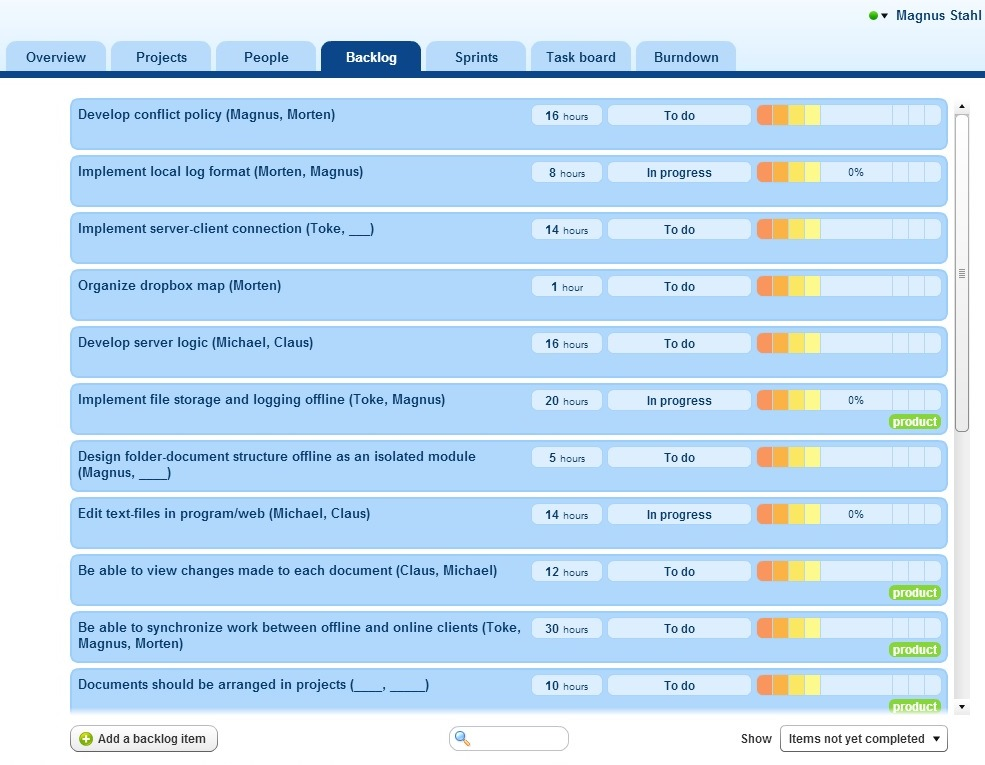
\includegraphics[width=\textwidth,natwidth=985,natheight=765]{illustrations/backlog1.jpeg}
  \caption{Backlog}
  \label{backlog1}
\end{figure}
\begin{figure}[H]
  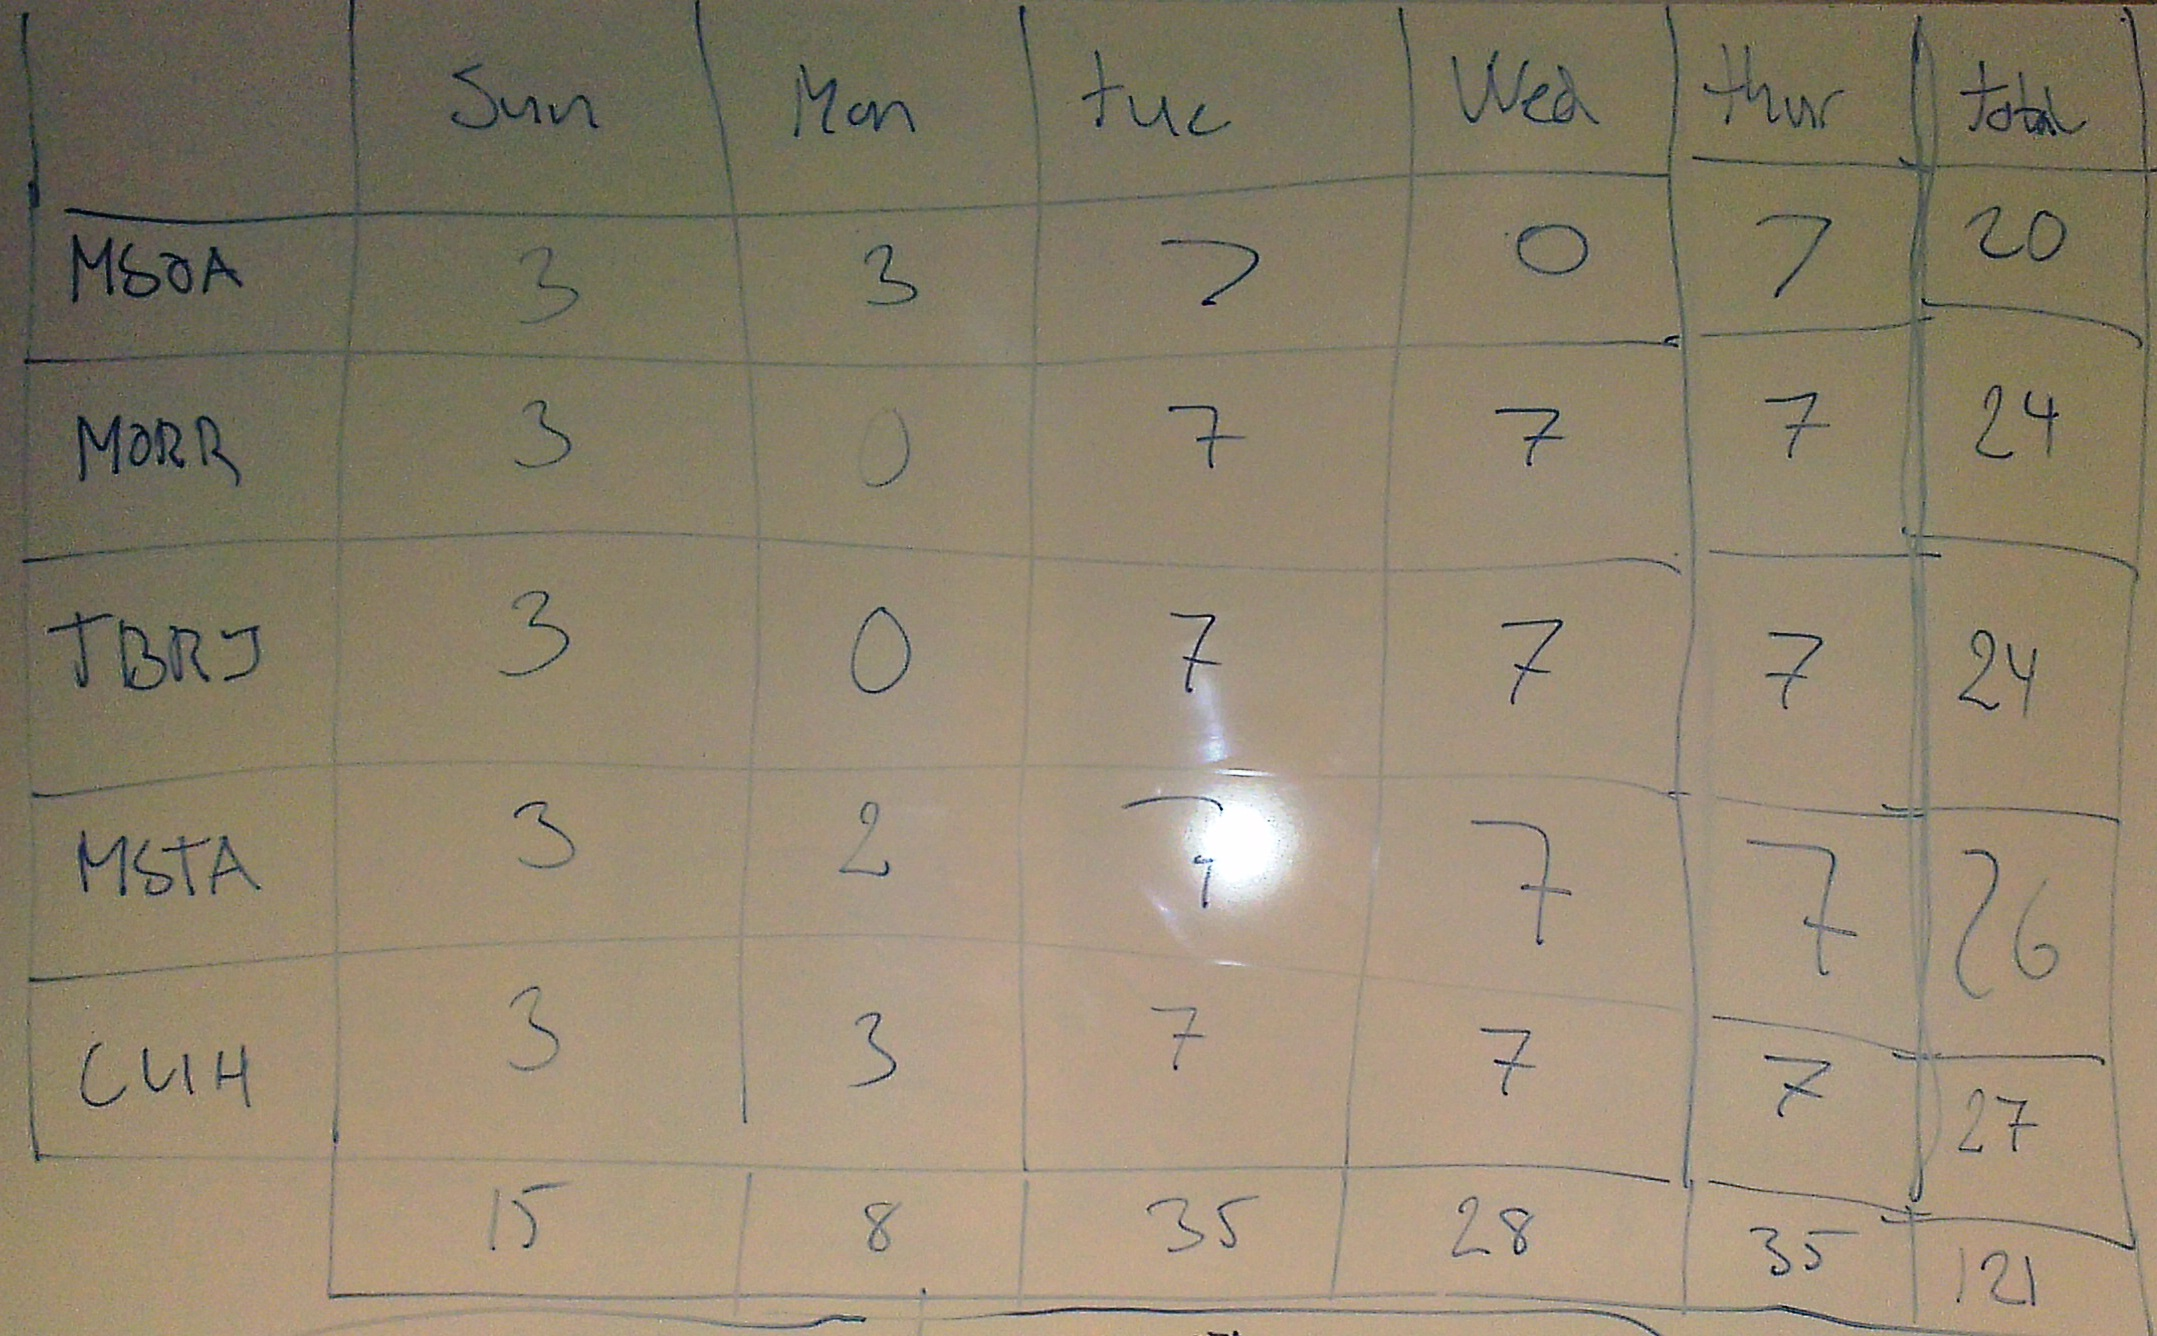
\includegraphics[width=\textwidth,natwidth=2157,natheight=1336]{illustrations/CapacityPlan.jpg}
  \caption{Capacity Plan}
  \label{capacityplan}
\end{figure}
\begin{figure}[H]
  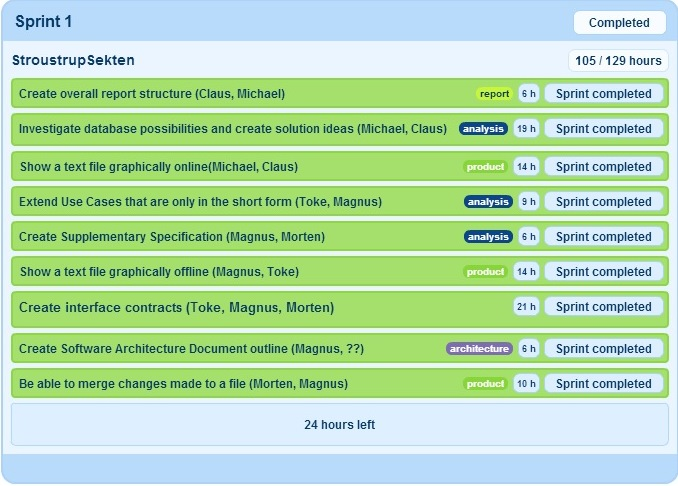
\includegraphics[width=\textwidth,natwidth=678,natheight=486]{illustrations/sprintbacklog1.jpeg}
  \caption{Sprint1 Backlog}
  \label{sprint1backlog}
\end{figure}
\subsection{Package Diagram}
\begin{figure}[H]
  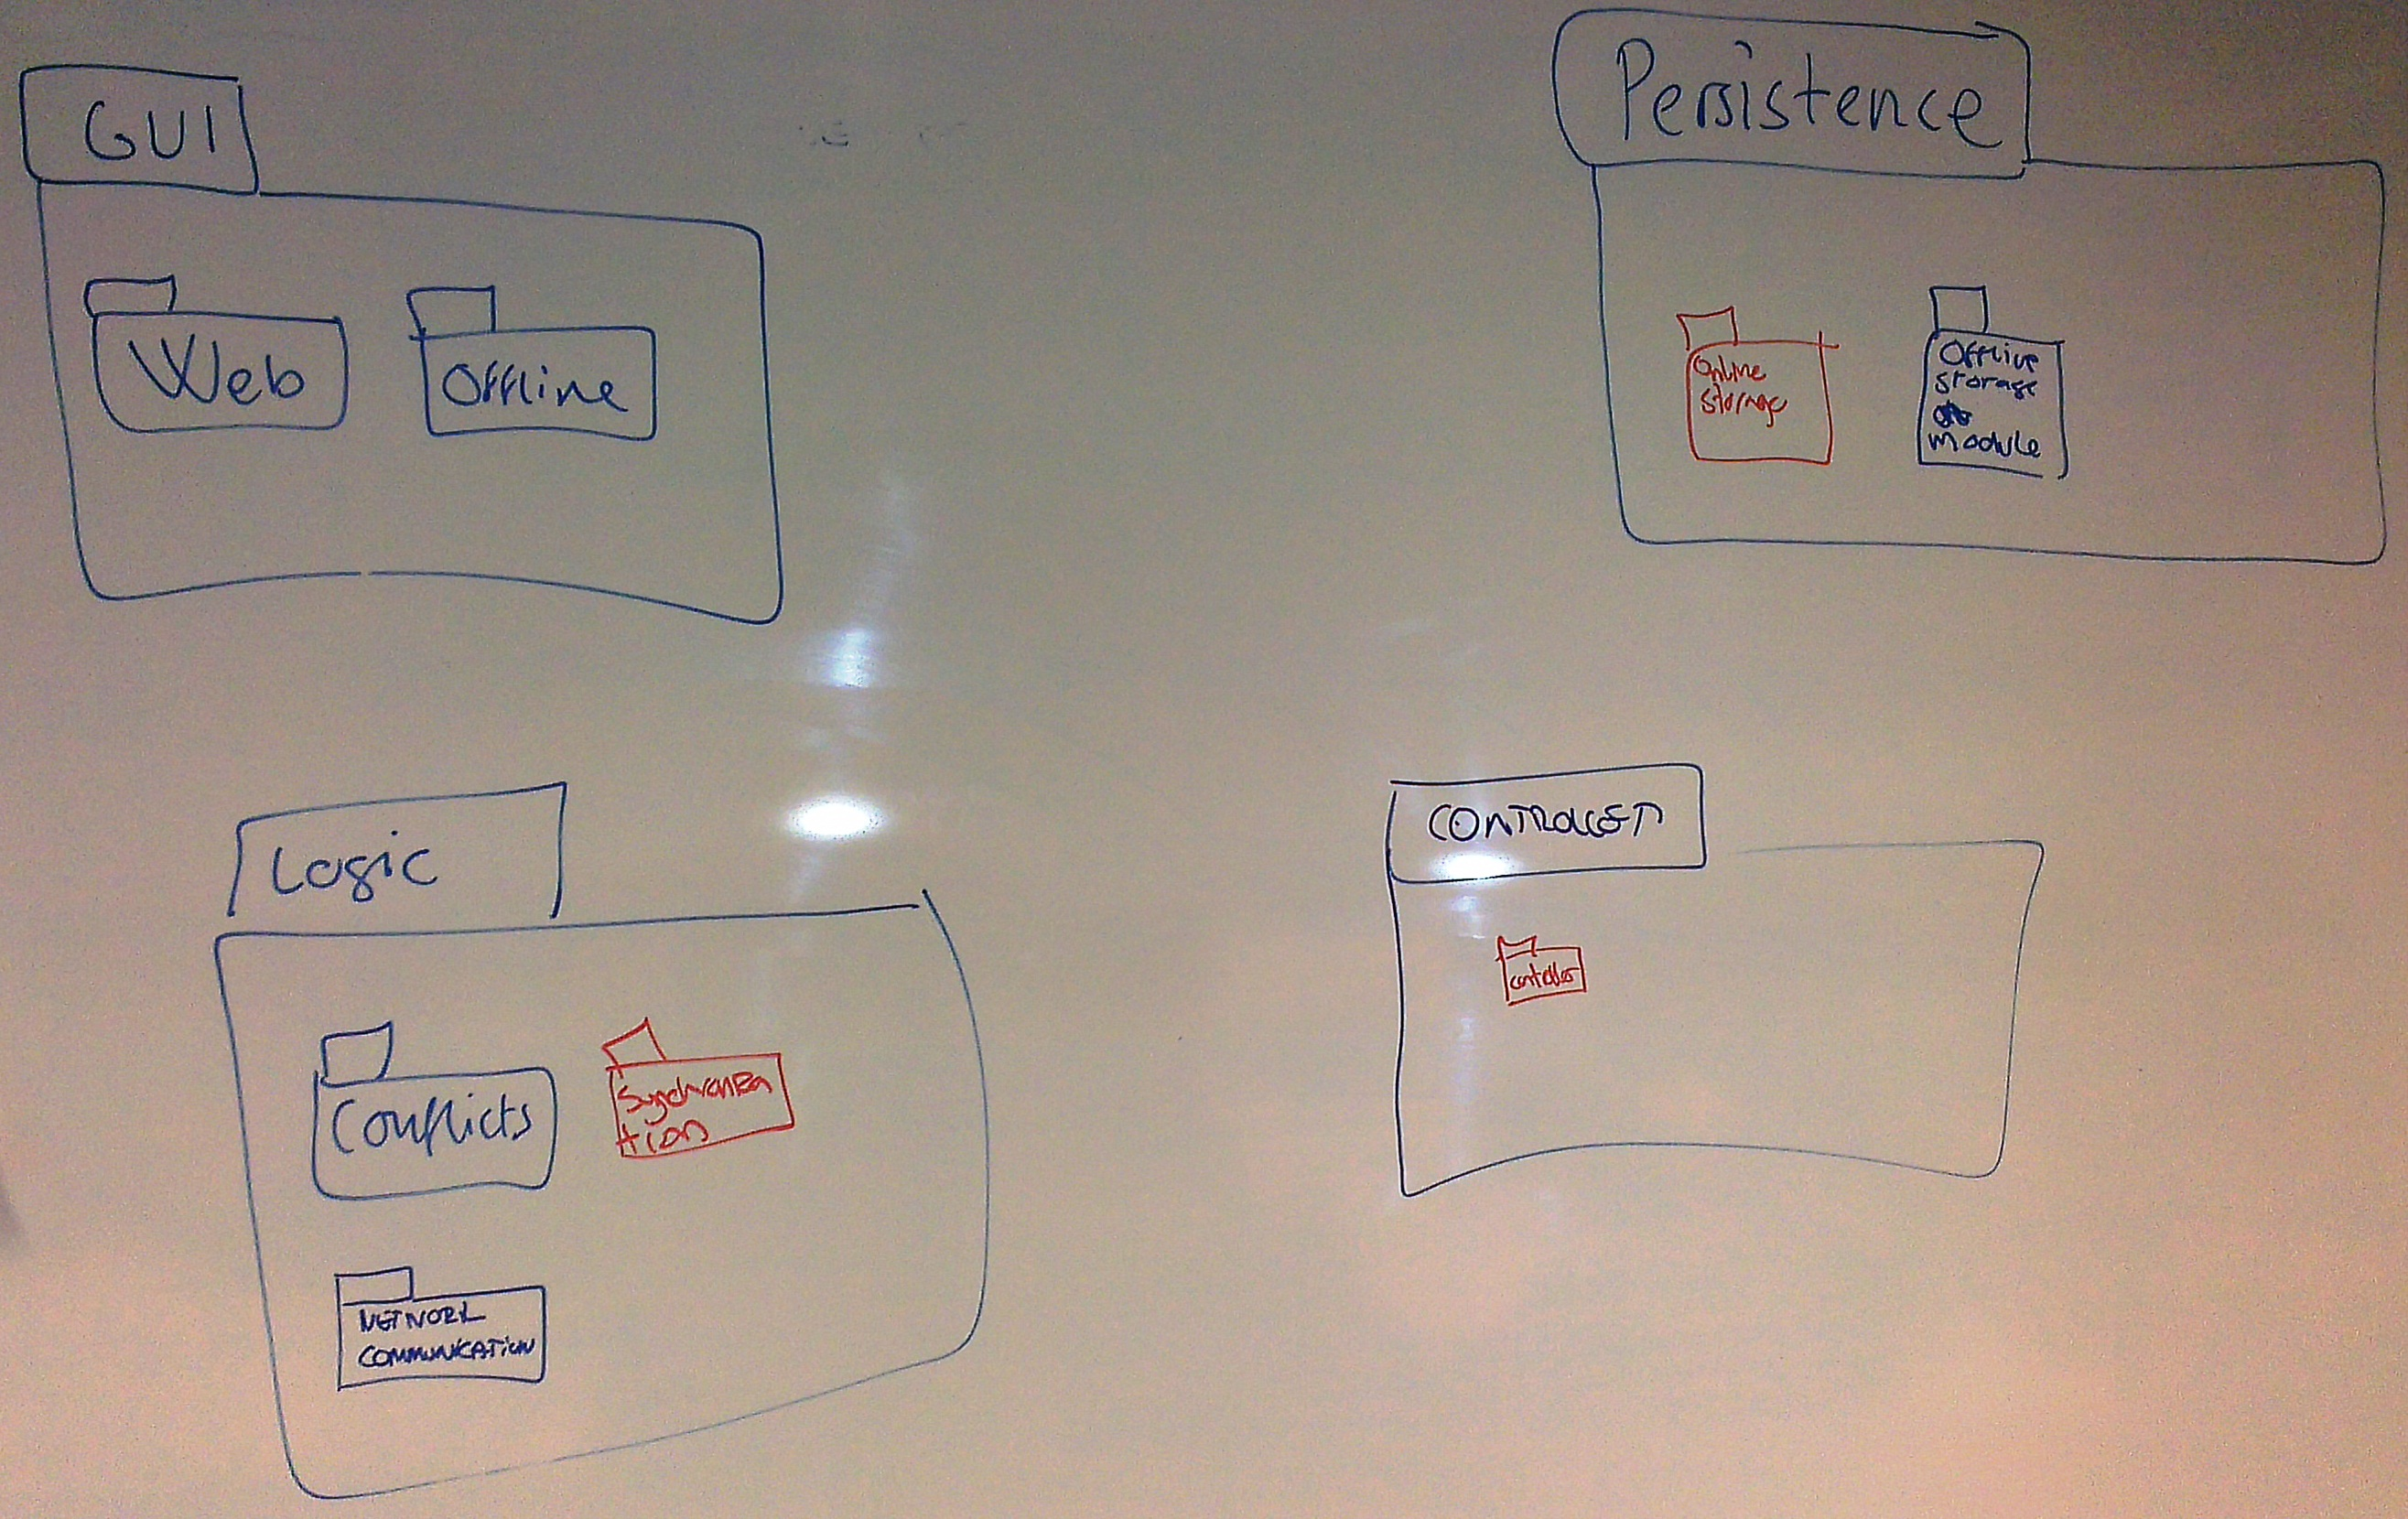
\includegraphics[width=\textwidth,natwidth=2631,natheight=1660]{illustrations/PackageDiagram.jpg}
  \caption{Package Diagram}
  \label{packagediagram}
\end{figure}
\subsection{Class Diagrams}
\begin{figure}[H]
  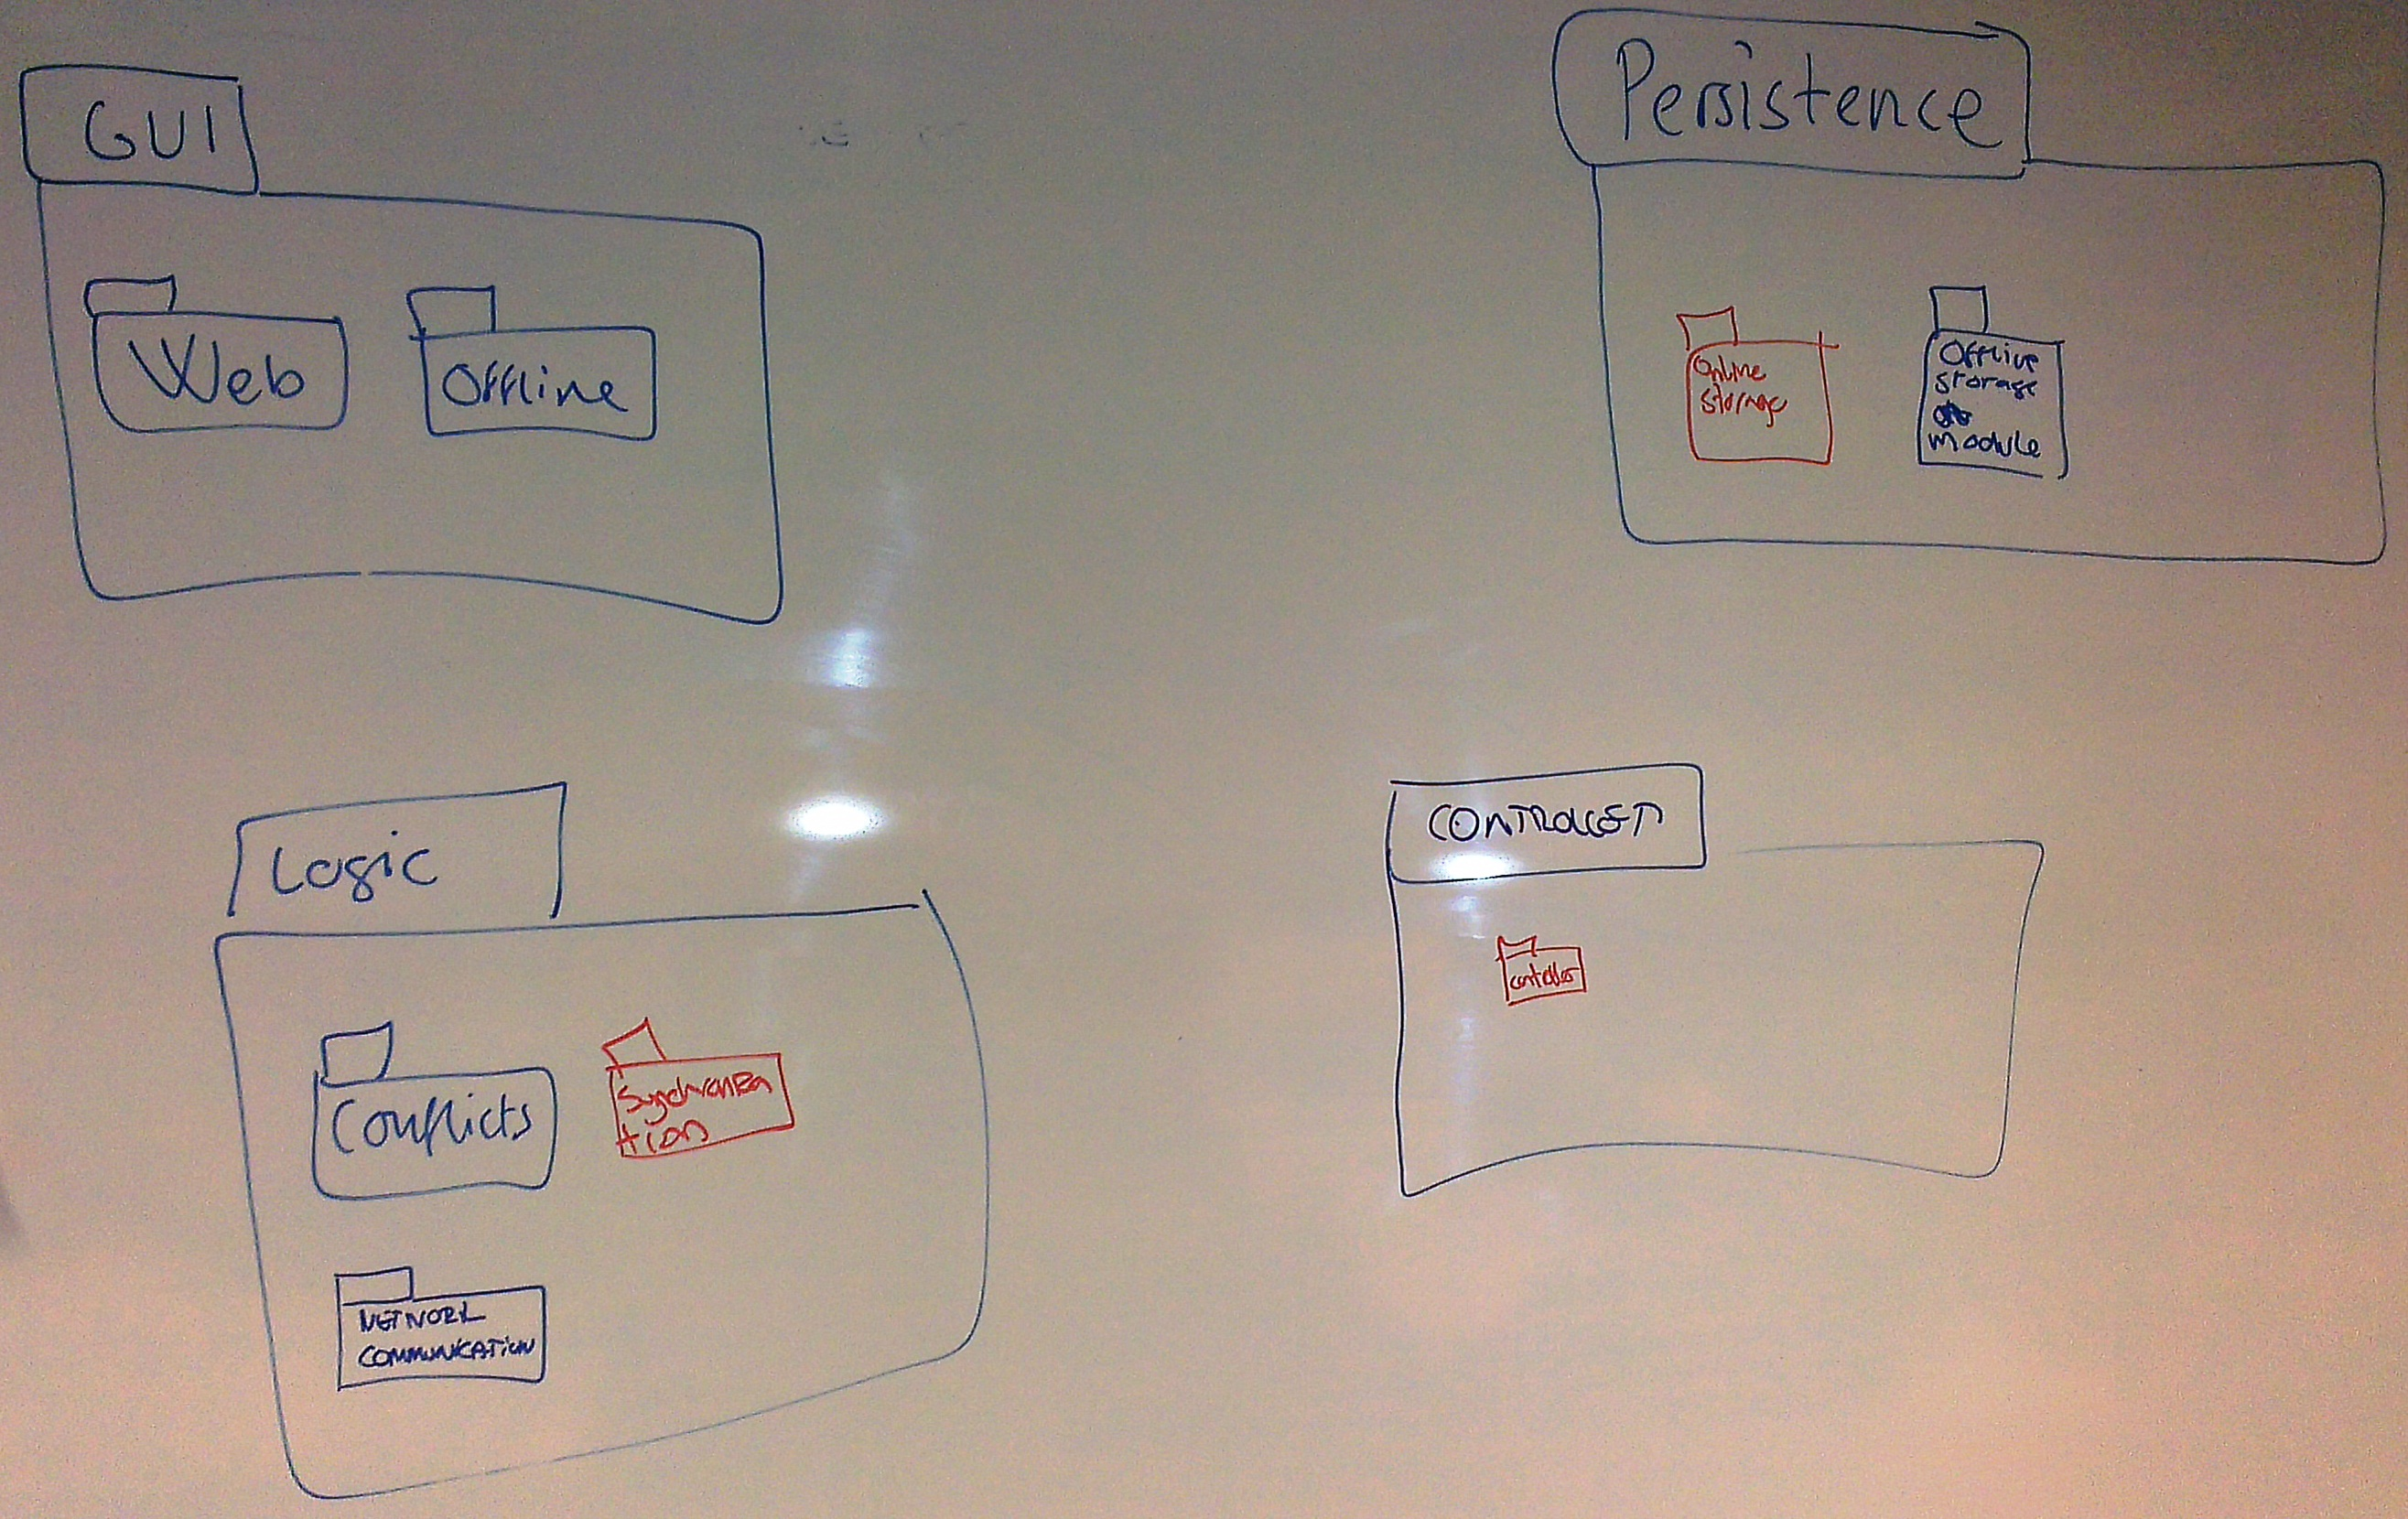
\includegraphics[width=\textwidth,natwidth=2631,natheight=1660]{illustrations/PackageDiagram.jpg}
  \caption{Class Diagram Server}
  \label{classdiagramserver}
\end{figure}
\begin{figure}[H]
  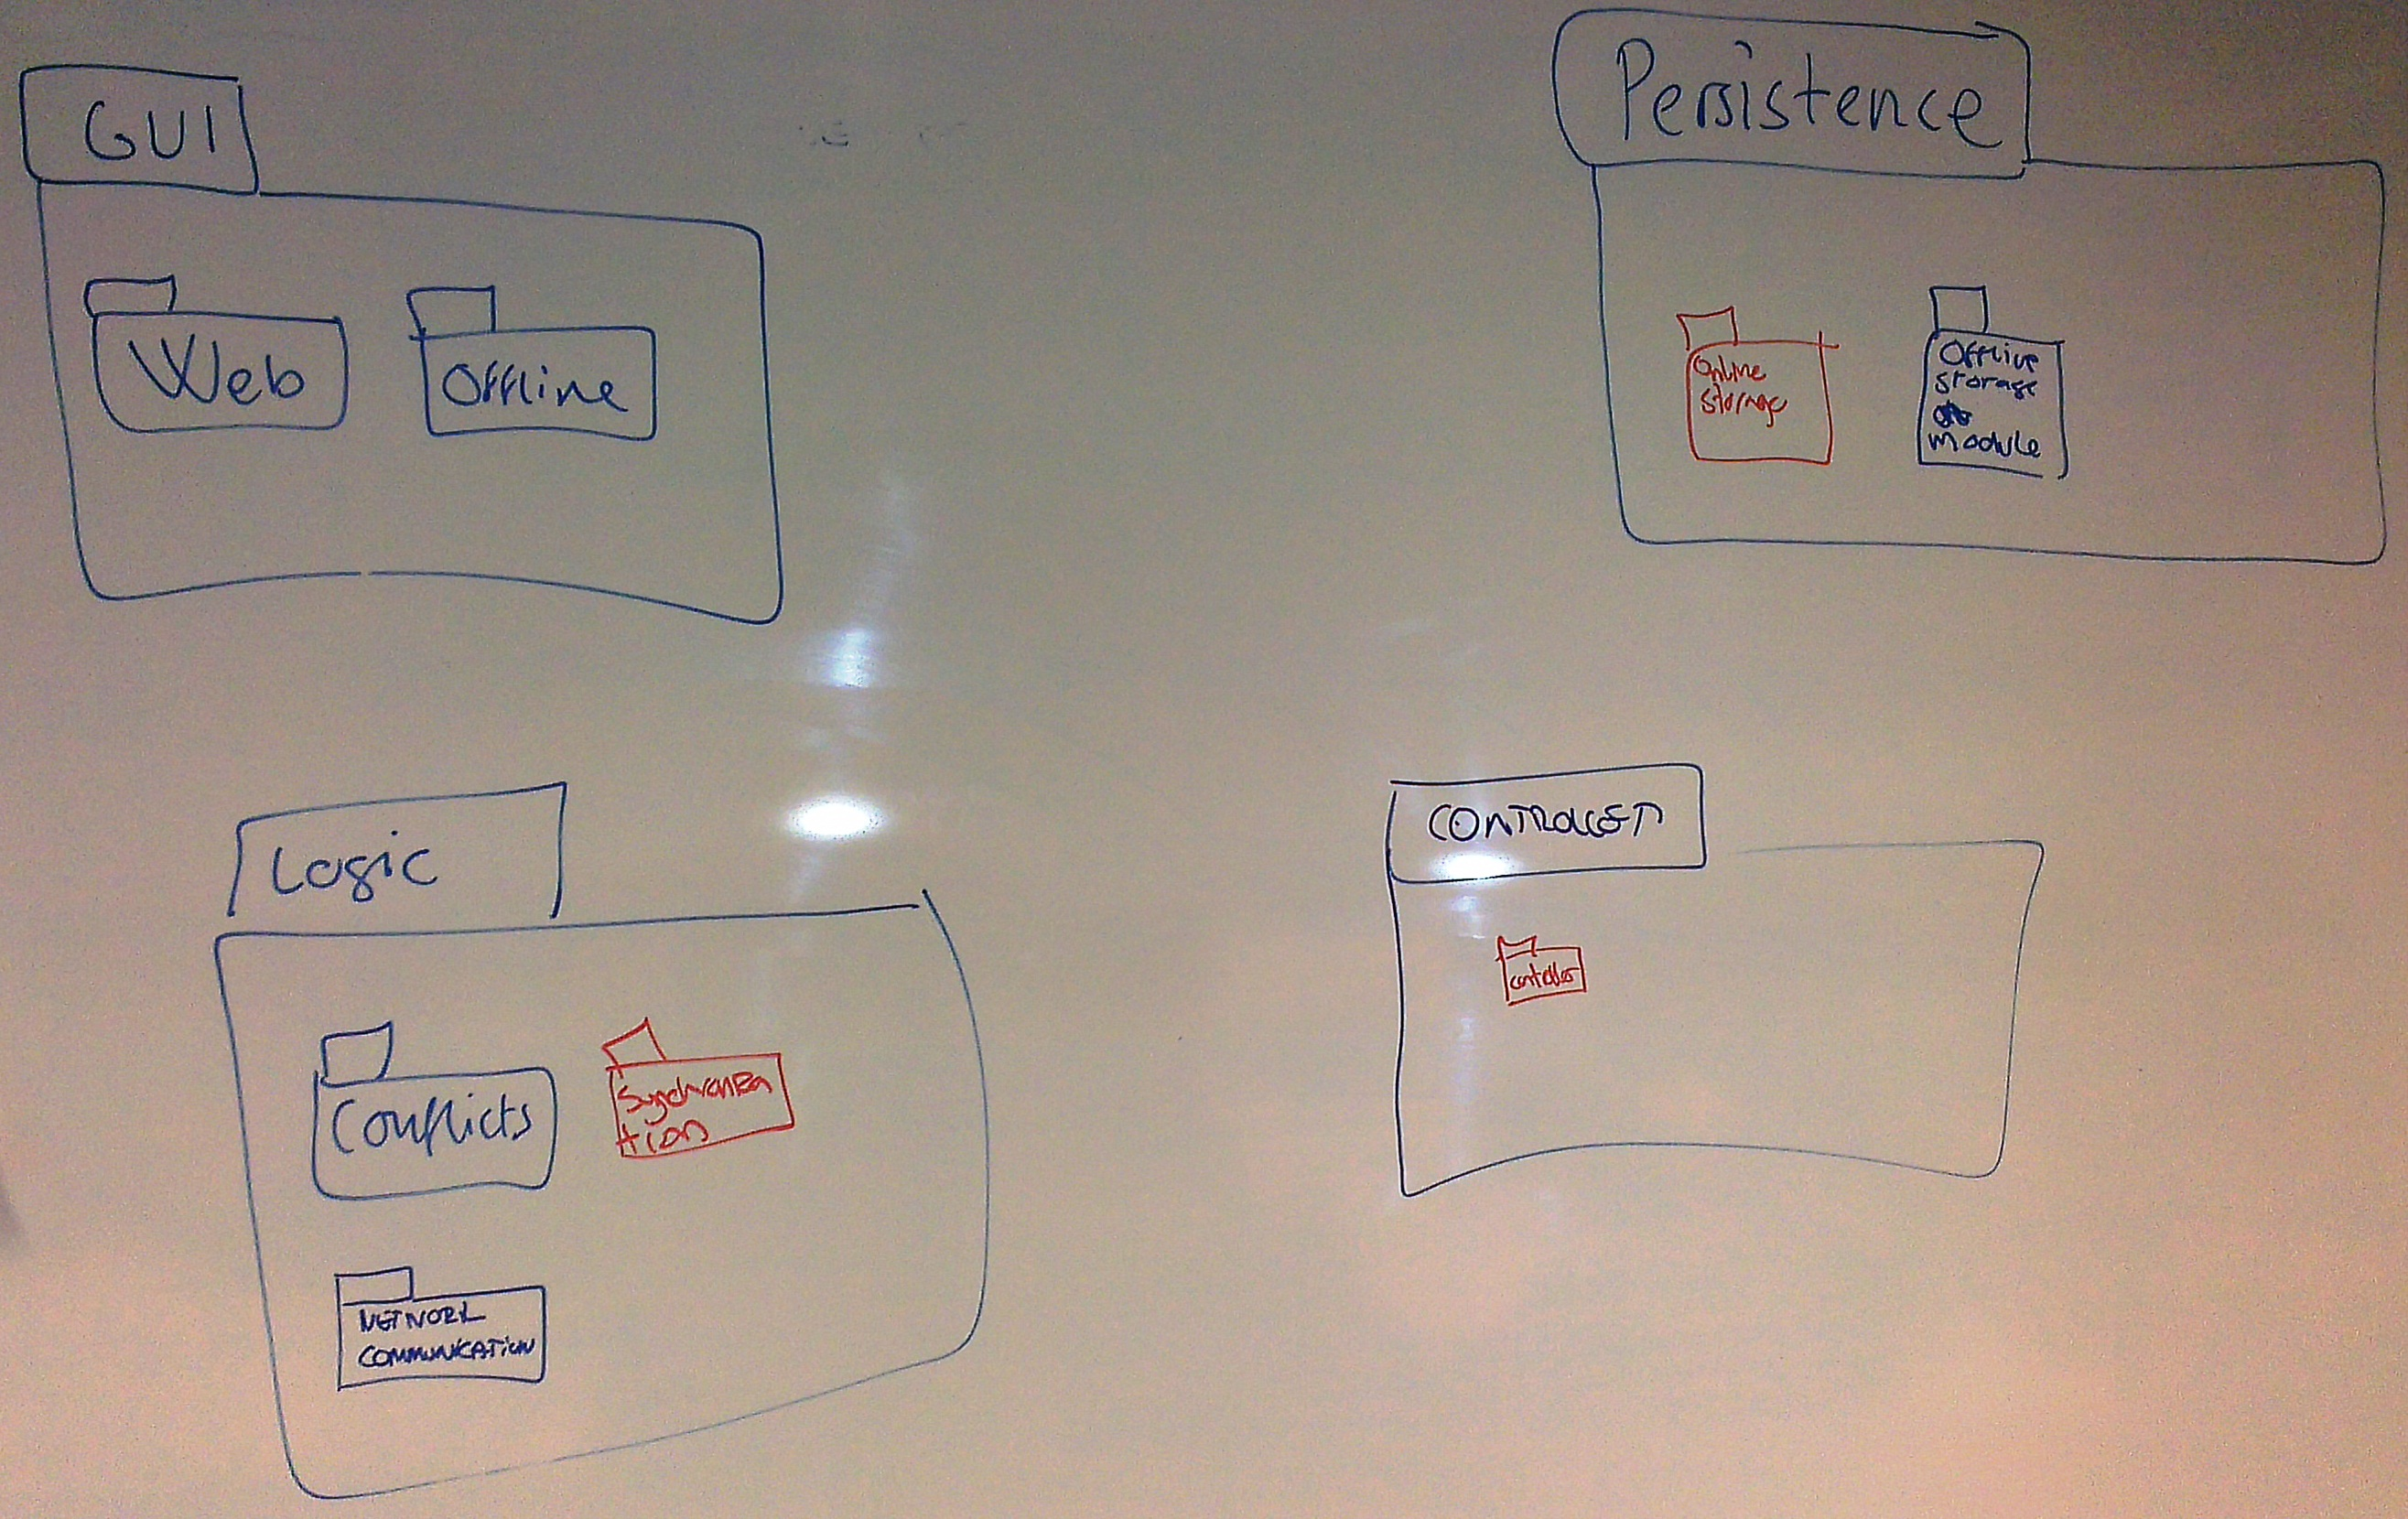
\includegraphics[width=\textwidth,natwidth=2631,natheight=1660]{illustrations/PackageDiagram.jpg}
  \caption{Class Diagram Client}
  \label{classdiagramclient}
\end{figure}
\subsection{E-R}
\begin{figure}[H]
  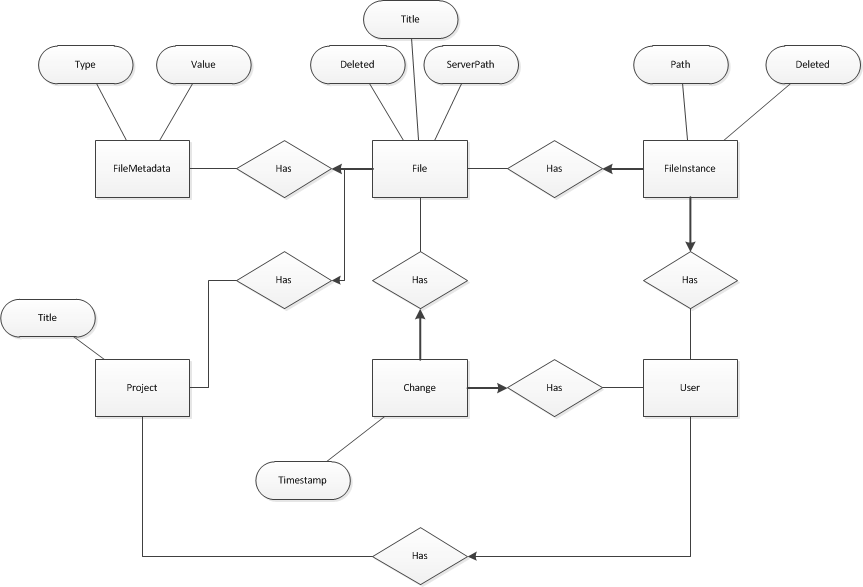
\includegraphics[width=\textwidth,natwidth=863,natheight=587]{illustrations/E-R.png}
  \caption{E-R Diagram}
  \label{erdiagram}
\end{figure}
\subsection{Sequence Diagrams}
% SDs
\subsection{Communication Diagrams}
\begin{figure}[H]
  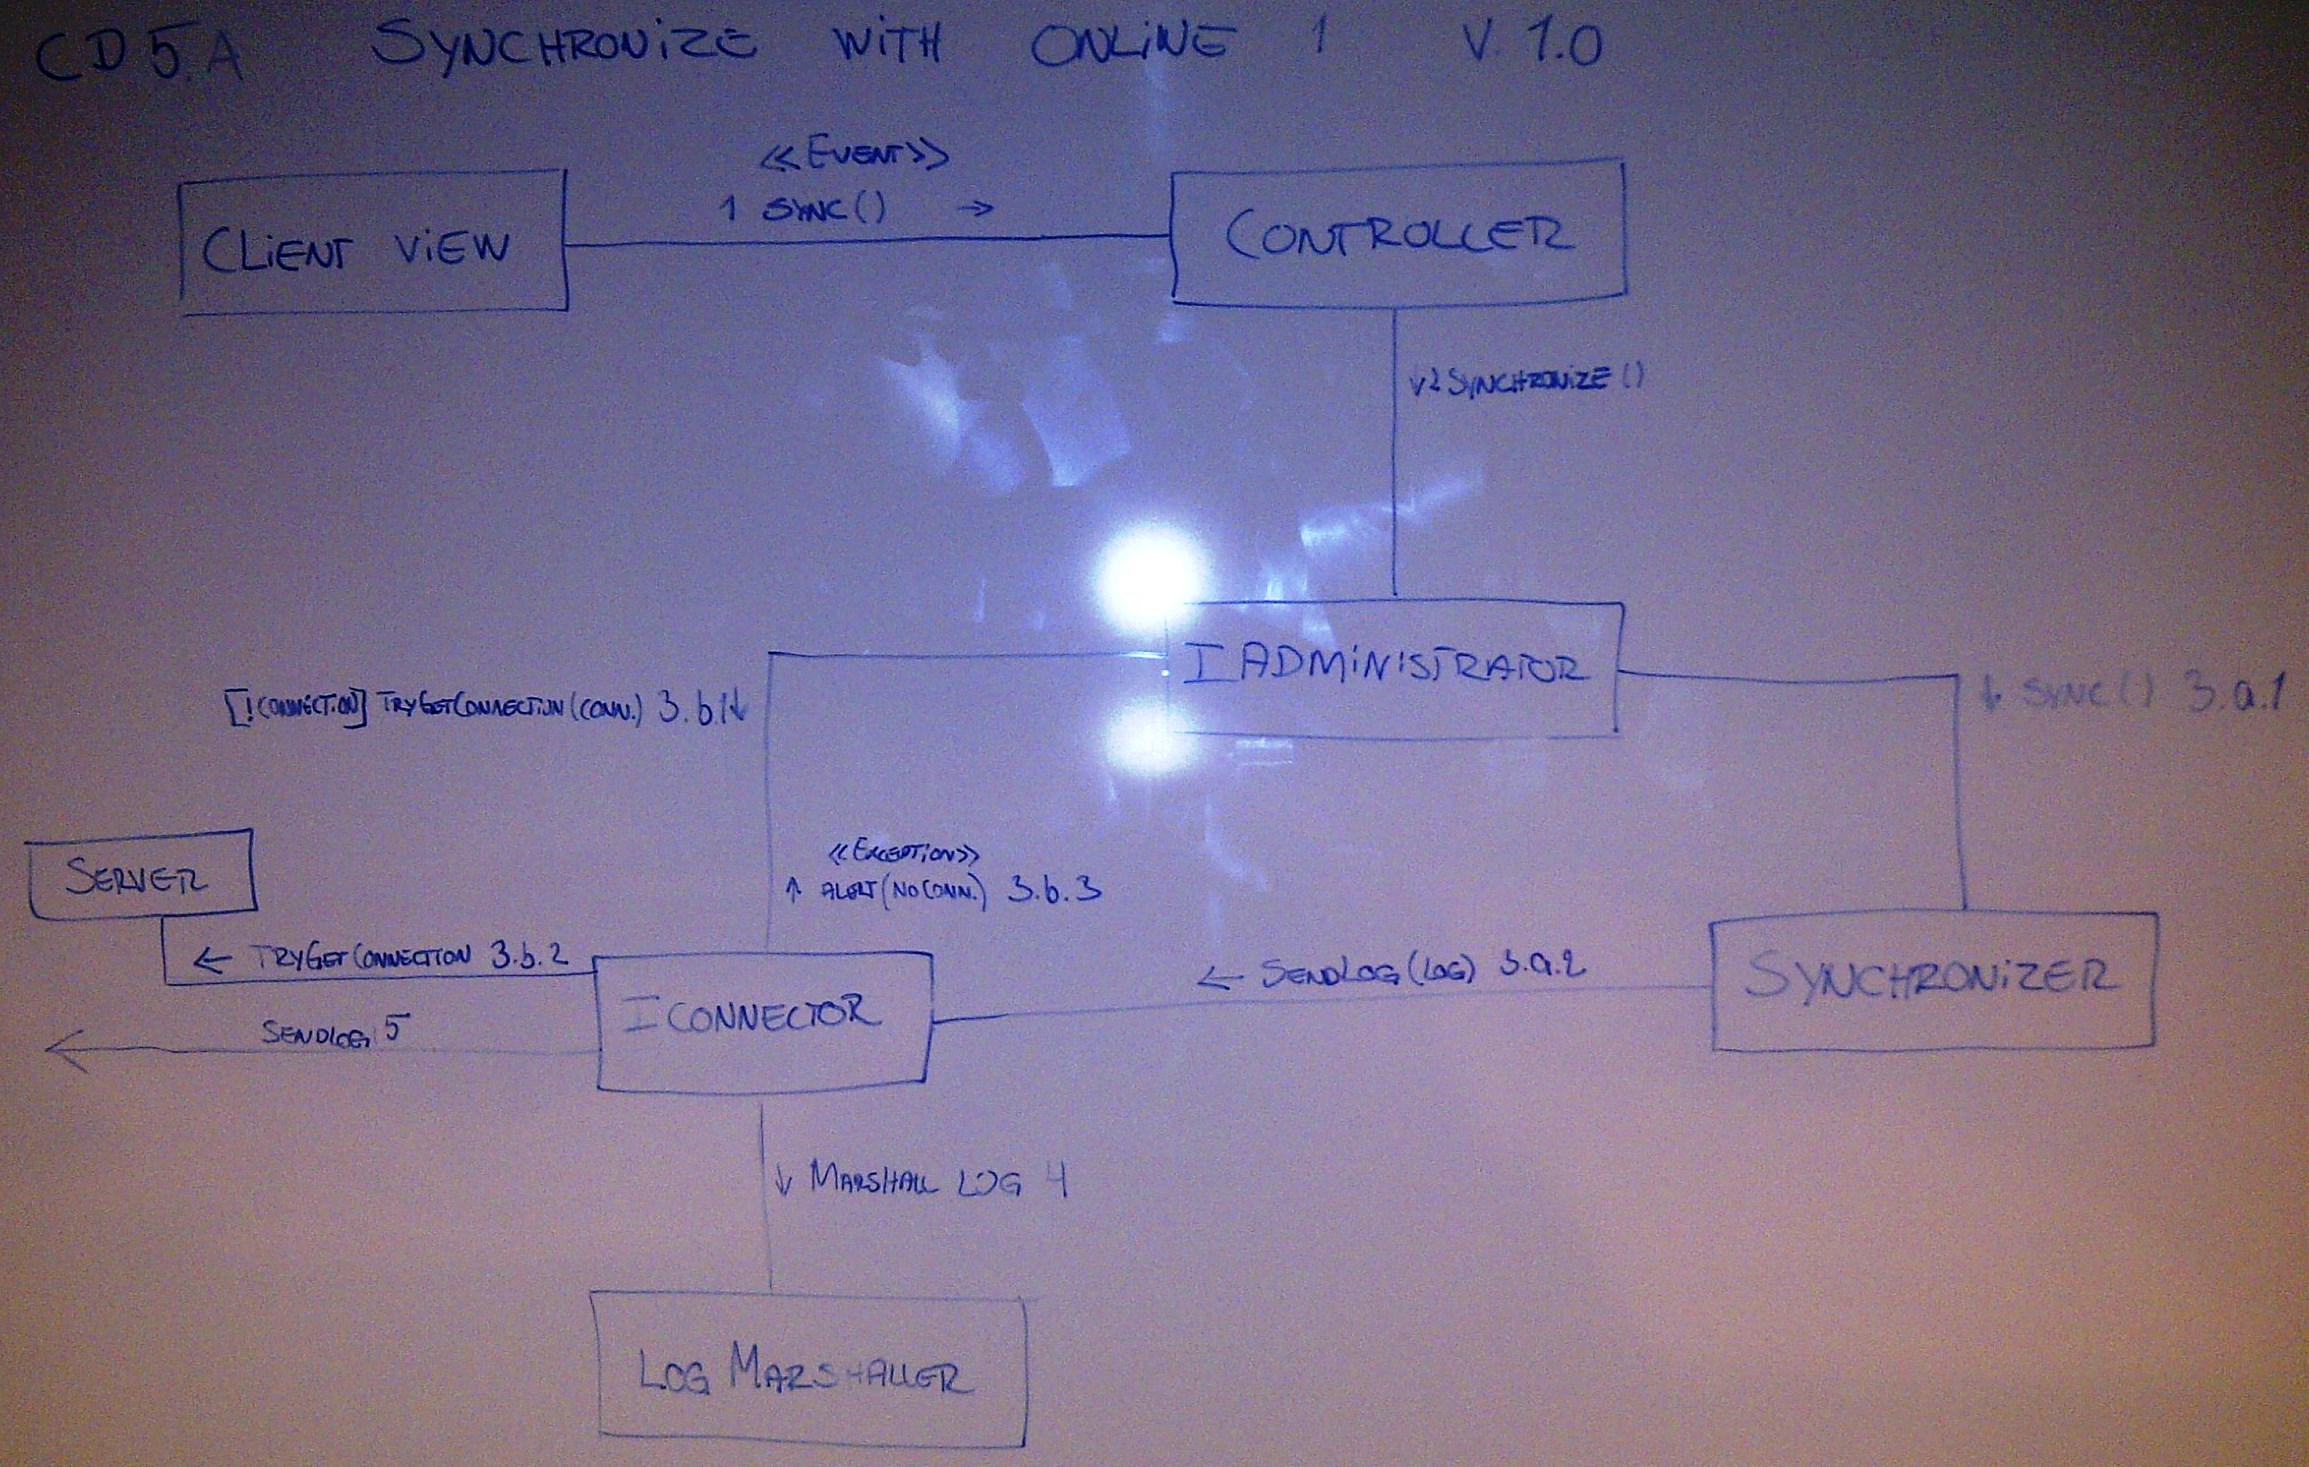
\includegraphics[width=\textwidth]{illustrations/CD5A.jpg}
  \caption{CD 5A}
  \label{CD5A}
\end{figure}
\begin{figure}[H]
  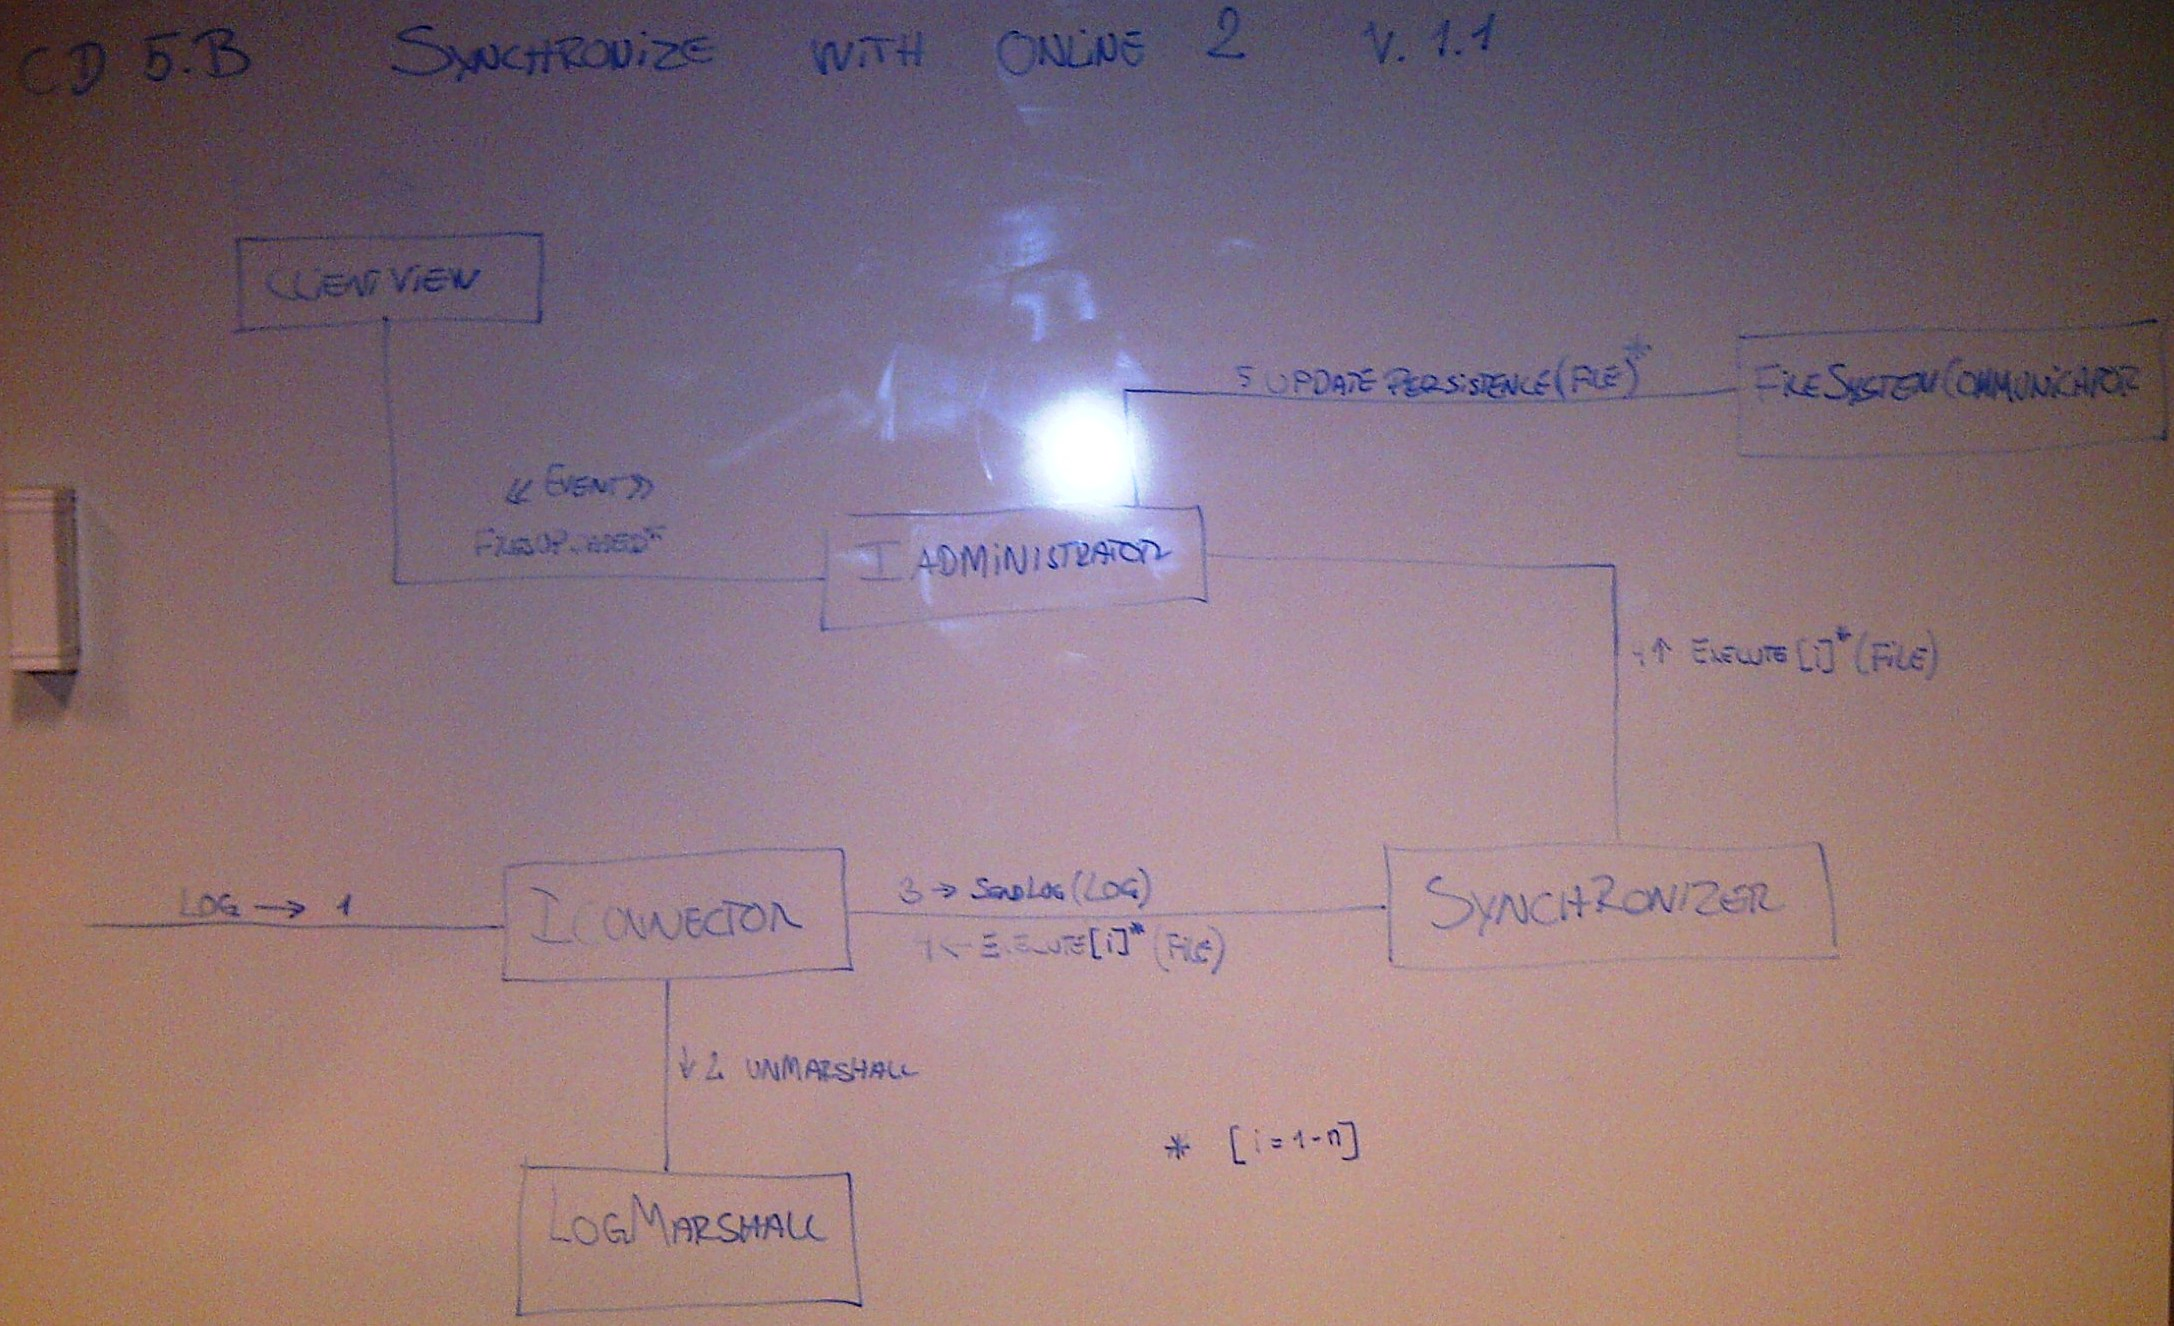
\includegraphics[width=\textwidth]{illustrations/CD5B.jpg}
  \caption{CD 5B}
  \label{CD5B}
\end{figure}
\begin{figure}[H]
  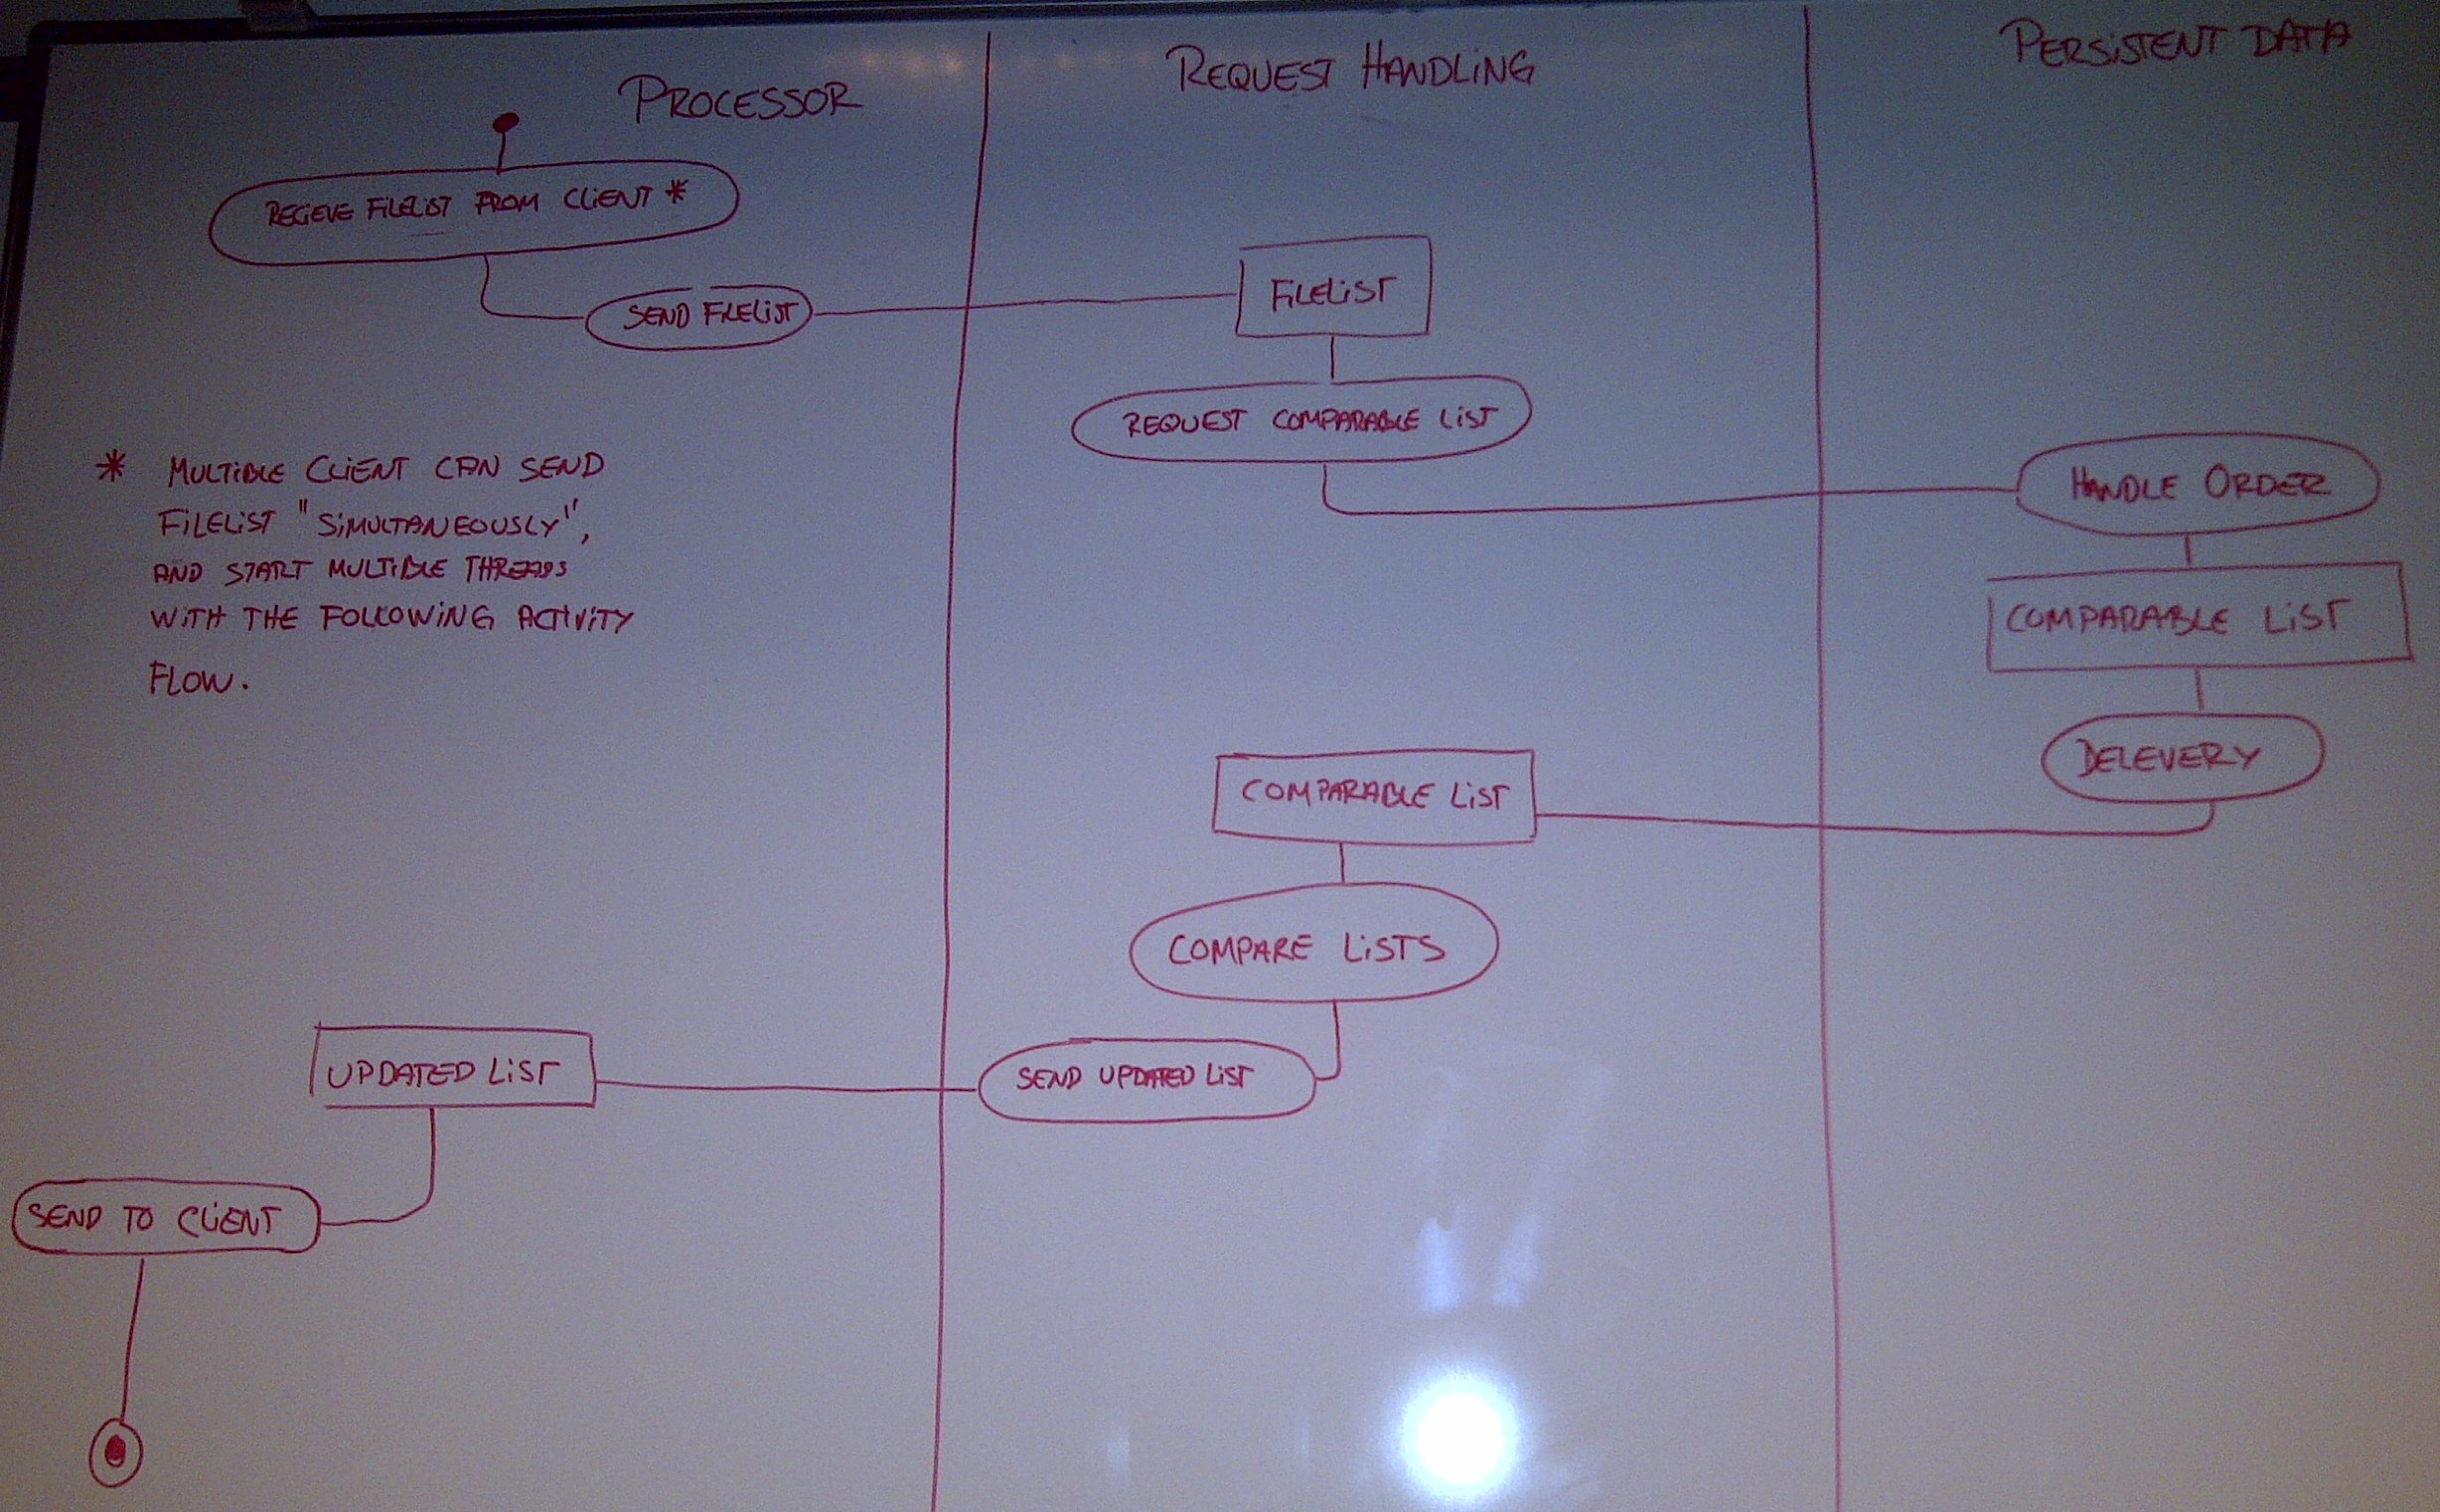
\includegraphics[width=\textwidth,natwidth=2456,natheight=1522]{illustrations/ActivityDiagram.jpg}
  \caption{Activity Diagram}
  \label{activitydiagram}
\end{figure}
%That's all folks!
\newpage
\subsection{Software Architecture Document(SAD)}
\subsubsection{Introduction : Architectural Representation}
This Software Architecture Document(SAD) is meant to be a thorough introduction to the architectural decisions made while designing and implementing the Slice of Pie project @ ITU Fall 2012.
One should be familiar with the major decisions regarding the overall structure after reading this document. Please note that for time bounded reasons, this document only contain the parts of a full SAD that are relevant to our project. 
We have selected the architectural views we find relevant in our project and we’ll briefly define them here before going into detail in separate sections:
\begin{itemize}
\item Logical View: This view summarizes our package architecture as well a brief description of some major components. In this section, we’ll include a UML package diagram and a discussion of the Model-View-Controller pattern.
\item Process View: This view explains the processes and threads
\item Data View: This view explains our persistent data model. We’ll review how we map objects to our relational database and commonly used queries in the database. In this section, we’ll include a UP Data Model and an UML activity diagram(swimlane diagram) that shows our data flow.
\item Deployment View: This view briefly models our physical deployment of the programs. We’ll show network interaction between our components as well as the physical components that we’ll use at the demo presentation. This view will include a deployment diagram.
\item Use Case View: :Maybe we’ll write something here later: Summary of the most significant use-cases and their non-functional requirements. Interaction diagrams can be used and described (System Sequence Diagram)
\end{itemize}


% Add bibliography
\bibliographystyle{cell}
\bibliography{bib}
\end{document}
